% !TeX spellcheck = en_US
\RequirePackage{ifluatex, ifxetex} % these are for the portability of this example - can be omitted in any actual document made for a certain engine

\ifnum 0\ifxetex 1\fi\ifluatex 1\fi>0
\else
  % only needed for using Greek letters outside math when running PDFLaTeX - leave out otherwise
  %\PassOptionsToPackage{LGR}{fontenc}
  %\RequirePackage{textgreek}
\fi

% Own environment definitions.
\newenvironment{it} {\itshape}


\documentclass[globalnumbering,centeredcaptions]{tutthesis} % see appendix for list of options

\pagestyle{headings} % Adds titles to the header


% ifnameyear is defined to demonstrate both versions in a single file. You may leave it out and simply use one version throughout your file.
\newif\ifnameyear
\nameyearfalse



% ==============
% Basic packages
% ==============
% You should use these unless you really know what you're doing

\ifnum 0\ifxetex 1\fi\ifluatex 1\fi>0
\else\usepackage[utf8]{inputenc}
\fi

\usepackage[english,finnish]{babel} % The language of the thesis last

% If you are working with a minimal LateX distribution, you may have to install some extra packages. Make sure that at least babel-finnish (available in e.g. texlive-lang-european) and the basic fonts (e.g. texlive-fonts-recommended) are installed.

\usepackage{babelbib} % You should use this unless you are using biblatex. Add option fixlanguage if you're writing in English (the thesis writing guide is asymmetric, requiring Finnish theses to have e.g. 'eds.' for sources in English, while requiring English theses to have all such parts in English)

\ifnameyear\usepackage{natbib} % add option longnamesfirst if you want to have full author list with first citation
\else\providecommand{\citep}{\cite} % This template is written using \citep to get name-year citations right, and in numerical mode the command is here aliased to the standard \cite. If you use numbered citations, leave this out and use \cite
\fi

% Path to search graphics used in this document.
\graphicspath{pictures/}


% ===============
% Useful packages
% ===============
% Packages which are not required for a thesis that follows guidelines, but may be convenient or necessary in common cases

%\usepackage{microtype} % subtle but nice improvements to how text is printed

%\usepackage{textcase} % may be used to keep parts of title lowercase
\usepackage{array}
\usepackage{tabularx} % e.g. multiline cells
\usepackage[shortcuts]{extdash} % add \- shortcut for hyphenation
\usepackage[export]{adjustbox} % package to adjust image positions
\usepackage{ltablex} % multi page table for abbreviations
%\usepackage{calc} % for performing length arithmetic such as column width = text width minus some other width
%\usepackage{longtable} % for tables spanning multiple pages

%\usepackage{psfrag} % editing ps files
%\usepackage{subfig} % parallel small figures a,b,c,...
%\usepackage{rotating} % for rotating e.g. full-page figures

%\usepackage{siunitx} % nice formatting for combinations of number and unit
\usepackage{amsopn} % For operator names; not necessary if amsmath is used
%\usepackage[fleqn]{amsmath} %Extensions to math handling; if you use this, you should use e.g. gather instead of equation due to a hyperref bug

\usepackage{listings} %Typesetting code
%\lstset{basicstyle=\footnotesize\ttfamily, numbers=left}
\renewcommand{\lstlistingname}{Ohjelma} % Rename "Listing" to "Ohjelma".
% If you want non-ASCII characters (e.g. in comments), check out the listingsutf8 package

\ifnum 0\ifxetex 1\fi\ifluatex 1\fi>0
  \usepackage[math-style=ISO]{unicode-math} %must not precede amsmath and most other math and font related packages
\else
  %\usepackage{bm} % The \bm command is used for bold italic variables used in some fields not to be used with unicode-math
  %\usepackage[helvratio=1]{newtxtext} \usepackage{newtxmath}% some recommend the newtx fonts
  \usepackage{textcomp} % symbols like \textdegree
\fi


% ===========================
% Bibliographic information
% ===========================
% These must be set before loading pdfx or beginning document
\author{Mauri Mustonen}
\title{sähköaseman älykkään elektroniikkalaitteen viestien tilaus ja prosessointi}
\datesubmitted{2018}{5}{17} % year, month, day; no leading zeroes; submitted for bachelor's theses and thesisapproved for master’s
\thesistype{Diplomityö} % Do not use ASCII apostrophe ' as it will not be substituted with the correct one (’) in the PDF metadata. Note that there are both short version (this) and a long one - "Master’s" vs. "Master of Science"
\major{Ohjelmistotuotanto}
\programme{Tietotekniikan koulutusohjelma} % Note apostrophes on all fields for PDF metadata
\examiner{Professori Kari Systä} %\and for plural
\datetopicapproved{2018}{8}{8}
\keywords{IEC 61850, MMS, AMQP, IED, sähköasema, älykäs elektroniikkalaite, ohjelmistokehitys, hajautettu järjestelmä, kommunikointiparadigmat}


% Packages that need to be loaded late
% ----------------------------------------------
% \usepackage[a-2u]{pdfx} % If you're using PDFLatex and your version of pdfx is not recent enough, you may run into the inputencoding bug. In that case, load inputenc after pdfx (and replace any non-ASCII characters in the metadata with e.g. \"{a})

\usepackage{hyperref} % This must (usually) be the last package you load - load this OR pdfx (which also loads hyperref). Usage of pdfx would be nice, but if you have issues with that you may fall back to just hyperref

\hyphenation{att-ri-buut-ti-en -nä-ky-vyys-a-lu-ees-sa}

\begin{document}


\maketitle
%First, the abstract in the language of the thesis (no language selection). Note that most fields are already defined.
\thesisdescription{Diplomityö}


\begin{abstract}
Sähkönjakeluverkko on tärkeä osa nykyistä yhteiskuntaa ja sen päivittäistä toimintaa. Sähköverkko koostuu sähköntuotantolaitoksista, sähkölinjoista ja sähköasemista. Sähköverkon eri komponenttien avulla sähkö toimitetaan tuontantolaitoksesta kuluttajille. Sähköasemat ja niiden automatisointi ovat tärkeässä roolissa verkon yleisen toiminnan ja turvallisuuden takaamiseksi. Tässä diplomityössä keskitytään suunnittelemaan ja toteuttamaan yksittäinen ohjelmistokomponentti osaksi isompaa sähköasemiin liittyvää järjestelmää. Suunniteltavan komponentin tarkoituksena on tilata tietoa sähköasemalta verkon yli ja saada jaettua tämä tieto järjestelmän muille komponenteille. Sähköasemalta tuleva tieto on esimerkiksi mittaustietoa ja mittaustiedosta kiinnostunut järjestelmän komponentti tarvitsee tämän tiedon käyttöliittymässä näyttämiseen.

Sähköasemilta tieto tilataan \emph{älykkäiltä elektroniikkalaitteilta} (engl. \emph{Intelligent Electronic Device}, \emph{IED}). IED:t ovat sähköaseman automaatiolaitteita, jotka on kytketty aseman verkkoon. Näistä käytetään myös nimitystä suojarele. IED-laitteiden kommunikointiin liittyy vahvasti maailmanlaajuinen \emph{IEC 61850} -standardi (engl. \emph{International Electrotechnical Commission}). Standardi määrittää kuinka IED-laitteet kommunikoivat verkon yli ja mekanismit kuinka ulkopuolinen ohjelma voi tilata siltä viestejä.

Ennen työn aloitusta ohjelmasta oli toteutettu demo, joka todisti kokonaisuuden toimivuuden. Demototeutuksessa oli kuitenkin ongelmia, jotka estivät sen käytön luotettavasti tuotannossa. Tässä työssä demoa käytettiin pohjana uuden version suunnittelulle. Demosta analysoitiin sen ongelmia ja mistä ne johtuivat. Näitä tietoja käytettiin uuden komponentin suunnitteluun liittyvissä päätöksissä.

Tuloksena työstä oli muusta järjetelmästä riippumaton ohjelmistokomponentti, joka pystyi tilaamaan viesteja IED-laitteelta IEC 61850 -standardin mukaisesti. Komponentti kykeni prosessoimaan ja jakamaan tilatut viestit järjestelmän muiden komponenttien kanssa. Komponentti päätyi tuotantoon osaksi muuta järjestelmää.
\end{abstract}


%Then, the abstract in the other language (explicit language selection) except for bachelor's theses
\begin{otherlanguage}{english}

\title{Substation’s intelligent electronic device messages subscription and processing}
\programme{Master’s Degree Programme in Information Technology}
\thesisdescription{Master of Science thesis}
\major{Software Engineering}
\examiner{Prof. Kari Systä}
\keywords{IEC 61850, MMS, AMQP, IED, substation, intelligent electronic device, software development, distributed system, communication paradigms}

\begin{abstract}
The abstract is a self-contained, concise description of the thesis: what was the problem, what was done, what was the result.
Do not include charts or tables in the abstract.
\end{abstract}
\end{otherlanguage}


\chapter*{Alkusanat}
\label{ch:alkusanat}

\begin{it}
	Mistä tämän diplomityönaiheen sain ja kiittää eri ihmisiä ketä työssä oli sidoshenkilöinä.
\end{it}

\vspace{2\baselineskip}

Tampereella, 19.4.2018

\vspace{2\baselineskip}

Mauri Mustonen


% Create table of content.
\tableofcontents


% List of figures and tables.
\listoffigures
\listoftables


\chapter*{Lyhenteet ja merkinnät}
\label{ch:lyhenteetjamerkinnat}

% This is not a "proper" table, so no table environment
% Suppressed left colsep; 20% - 1 x colsep; right colpsep; left colpadding; 80% - 1 x colpadding; suppressed right colpadding
\begin{tabular}[h]{@{} p{0.2\textwidth-\tabcolsep} p{0.8\textwidth-\tabcolsep} @{}}
	AMQP & engl. \emph{Advanced Message Queuing Protocol} \\
	FFI & engl. \emph{Foreign Function Interface}, mekanismi, jolla ajettava ohjelma voi kutsua toisella kielellä implementoitua funktiota\\
	GIL & engl. \emph{Global Interpreter Lock}, tulkattavassa kielissä oleva globaali lukitus, joka rajoittaa yhden säikeen suoritukseen kerrallaan \\
	HAL & engl. \emph{Hardware Abstraction Layer}, laitteistoabstraktiotaso abstraktoimaan laitteen toiminnalisuus lähdekoodista \\
	IED & engl. \emph{Intelligent Electronic Device}, konfiguroitava sähköaseman älykäs elektroninen laite, joka toteuttaa aseman toiminnallisuutta \\
	MMS & engl. \emph{Manufacturing Message Specification} \\
	RCB & engl. \emph{Report Control Block}, raporttien konfigurointiin ja tilaukseen tarkoitettu lohko asiakasohjelmalle \\
\end{tabular}

% Reset table counter because abbreviations incremented it already.
\setcounter{table}{0}

% Each chapter is it's own file and included here.
\chapter{Johdanto}
\label{ch:johdanto}
\begin{it}
	Kirjoita tähän johdantoa työstä ja aiheesta. Kuinka työ valittiin ja miksi tekijä valitsi tämän työn. Kirjoita myös mitä tehtiin. Kokonaiskuva työstä pitäisi saada johdannosta. Alusta lukijaa todella hyvin yleismaallisella kuvalla ja taustalla. Asiaa pitäisi olla hyvin hallussa ennen teoriaosuuteen siirtymistä.
\end{it}

\section{Tausta}

\section{Laajuus}

\section{Tavoitteet}
\chapter{IEC 61850 -standardi}
\label{ch:iec61850-theory}
% Aihepiirijärjestys tutusta uuteen.
% Tuttuja asioita: sähköasema, julkaisija-tilaaja-paradigma, viestejä voidaan tilata.
% Luvussa käsiteltävät asiat.
IEC 61850 -standardi määrittää säännöt, kuinka sähköaseman laitteet kommunikoivat keskenään verkon yli \cite[s.~1]{Kaneda2008}. Standardi koskee myös aseman kanssa kommunikoivia ohjelmistoja \cite[s.~10]{IEC61850-7-1}. Standardi on laaja monesta dokumentista koostuva kokonaisuus. Tämän takia tässä luvussa standardista käsitellään vain diplomityön kannalta tärkeitä asioita. Käsittely aloitetaan yleiskuvalla ja edetään tärkeään asiaan. Saatuja tietoja tullaan käyttämään myöhemmin pohjana järjestelmän arkkitehtuurin ja ohjelmiston suunnittelussa.


\section{Yleiskuva}
% Sähköaseman IED-laitteet toteuttavat aseman toiminnallisuutta.
Sähköaseman tehtäviin kuuluu mm. jännitteen muuntaminen, verkon jakaminen ja sen toiminnan tarkkailu. Virhetilanteissa aseman laitteisto toimii estääkseen suuremman vahingon. Näitä laitteita sähköasemalla ohjaa ja tarkkailee sen automaatiolaitteet, joita kutsutaan \emph{älykkäiksi elektroniikkalaitteiksi} (\emph{Intelligent Electronic Device}, \emph{IED}). IED:t ovat kytketty sähköverkon laitteisiin joita ne ohjaavat \cite[s.~63--64]{IEC61850-7-1}. Näitä laitteita on mm. muuntajat ja katkaisijat. IED:t myös kytketään verkkoon, jotta ne voivat kommunikoida keskenään ja asemalta ulospäin \cite[s.~31]{IEC61850-7-1}. Asemalta ulospäin kommunikointi mahdollistaa sen etäohjauksen ja tarkkailun ohjelmiston avulla \cite[s.~1]{Brunner2008}.

% Standardi IED-laitteiden kommunikoinnin määrittämiseen.
% Standardia voi toimia monella eri tekniikalla, mutta käytetään MMS-protokollan avulla.
IEC 61850 -standardi määrittää kuinka IED-laitteet ja etäohjelmistot kommunikoivat keskenään. Standardin tarkoitus on asettaa yhteiset säännöt, jotta eri valmistajien laitteet ja ohjelmistot olisivat yhteensopivia keskenään. Standardi on määritetty tekniikasta riippumattomaan muotoon, joka erikseen mallinnetaan halutulle tekniikalle \cite{IEC61850-1}. Mallinnuksia on olemassa eri tekniikoille, mutta tässä työssä kommunikointi tapahtuu pelkästään \emph{MMS}-protokollan (\emph{Manufacturing Message Specification}) päällä. MMS-protokolla on TCP/IP-protokollaperheen päällä toimiva kommunikointiprotokolla \cite{MMS-protocol-stack-and-API}.

% Viestien tilauksen pääpiirteinen toiminta.
Standardi määrittää säännöt kuinka asiakasohjelmat voivat tilata viestejä IED-laitteelta verkon yli. Viestien tilaus noudattaa julkaisija-tilaaja-paradigmaa, jossa IED-laite on julkaisija ja asiakasohjelmat tilaajia. Julkaisija-tilaaja-paradigma käsiteltiin aikaisemmin kappaleessa \ref{ch:julkaisija-tilaaja-paradigma}. Viestien sisältö on IED-laitteessa olevaa tietoa, kuten mittausdataa tai siihen kytketyn laitteen tilatietoa. Viestit tilataan IED-laitteelta olevalta oliolta, joka konfiguroidaan ennen tilausta. Standardi asettaa rajoituksia tilaajien määriin, jotka täytyy ottaa huomioon ohjelmiston suunnittelussa. Jotta näitä rajoituksia ja tilauksen toimintaa voidaan ymmärtää, täytyy ensin tarkastella, kuinka standardi määrittää muuttujia IED-laitteeseen. \mbox{\cite[s.~91--97]{IEC61850-7-2}}


\section{Sähköaseman laiteiden mallinnus}
% Muuttujilla IED-laite mallintaa aseman laitetta.
Muuttujilla IED-laite mallintaa siihen kytkettyä sähköaseman laitetta kuten katkaisijaa tai muuntajaa. Muuttujat esittävät mm. linjasta mitattua jännitteen arvoa tai katkaisijan tilaa, joka voi olla auki tai kiinni. IED-laitteessa olevien muuttujien määrä vaihtelee sen mukaan mitä laitetta sen on tarkoitus ohjata. \cite[s.~28]{IEC61850-7-1}

% Muuttujat muodostuvat valmiiksi määritetyistä luokista.
Mitä muuttujia IED-laite sisältää määrittyy standardin mukaan. Standardi esittää luokkamäärityksiä kaikille sähköaseman laitteille mm. katkaisijoille ja muuntajille. Luokka määrittää mitä muuttujia sen instanssi tulee sisältämään jotka kuvaavat kyseistä laitetta. Luokasta muodostetaan instanssi IED-laitteelle sen mukaan, mitä laitetta se ohjaa. Esimerkiksi jos IED-laite ohjaa linjan katkaisijaa, määritetään IED-laitteeseen standardin määrittämä katkaisijaluokan instanssi. Tällöin IED-laite sisältää muuttujia katkaisimen tilasta ja sen ohjauksesta. \cite{IEC61850-7-3, IEC61850-7-4}

% Luokkat muodostavat hierarkian ja koostuvat toisistaan.
Standardin luokkamääritykset sisältävät aliluokkia, jotka vuorostaan sisältävät muuttujia tai muita aliluokkia. Standardissa luokkamääritykset toimivat samalla periaatteella kuin oliohjelmoinnin luokat. Luokat sisältävät samaan asiaan liittyviä muuttujia ja toiminnallisuutta. Näistä luokista ja muuttujista standardissa muodostuu oliopohjainen hierarkkinen rakenne. Esimerkiksi muuntajaa mallintava luokka sisältää aliluokkia mittaustiedon esittämisestä. Samaa aliluokkaa käytetään jonkin muun mittaustietoa sisältävän laitteen mallintamiseen. Voidaan sanoa, että standardin mukainen laitteen luokka koostuu muista aliluokista. Kun laitteen mallintavasta luokasta tehdään instanssi IED-laitteelle, samalla myös tehdään instanssi kaikista sen aliluokista. IED-laite siis sisältää myös kaikki aliluokkien muuttujat. \mbox{\cite[s.~108]{IEC61850-7-1}}

\section{Muuttujien yksilöinti IED-laitteessa}
% Viittaus muuttujiin hierarkiassa.
IED-laite siis sisältää muuttujia hierarkiassa sen mukaan mitä laitetta se ohjaa. Näitä muuttujia voidaan lukea ja kirjoittaa standardin määrittämillä palvelukutsuilla. Jotta voidaan yksilöidä mitä muuttujia halutaan kutsulla lukea tai kirjoittaa, pitää niitä pystyä yksilöimään hierarkiassa. Tätä varten standardi määrittää viittaustekniikan, jota käytetään kutsun yhteydessä yksilöimään mitä muuttujia se koskee. Tämä viittausformaatti on määritetty kuvassa \ref{fig:iec61850-data-reference}. Viittaus muodostuu hierarkiassa olevien luokkien instanssien ja muuttujien nimistä. Nimiä yhdistetään peräkkäin, jolloin viittausta voidaan seurata lukemalla minkä luokan instanssin mitä muuttujaa halutaan lukea tai kirjoittaa. Ensimmäisen ja toisen nimen väliin tulee kauttaviiva (/) ja loput yhdistetään pisteellä (.). \mbox{\cite[s.~625--626]{Mackiewicz2006}} \mbox{\cite[s.~93--95]{IEC61850-7-1}}

\begin{figure}[ht!]
	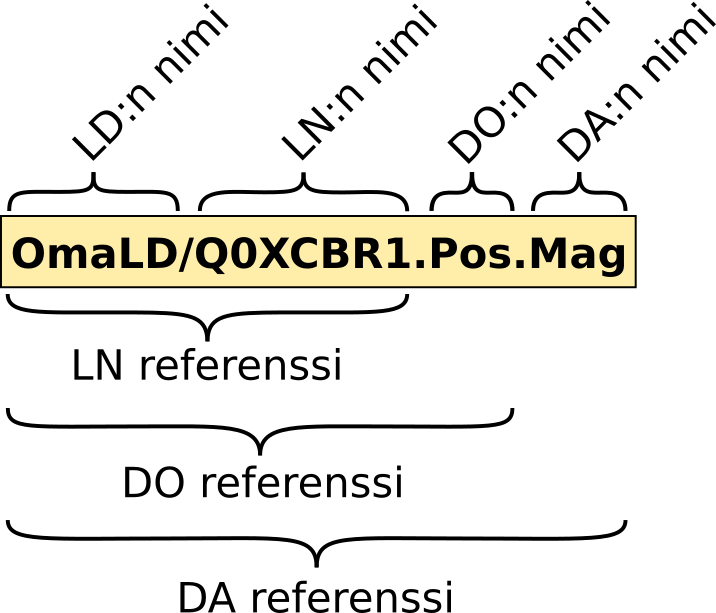
\includegraphics[width=0.5\textwidth]{pictures/iec61850-data-reference.png}
	\caption{IEC 61850 -standardin määrittämä viitteen rakenne (pohjautuu kuvaan \mbox{\cite[s.~93]{IEC61850-7-1}}).}
	\label{fig:iec61850-data-reference}
\end{figure}

% Viittauksen käsitteet lyhyesti.
Viite muodostuu käsitteistä:
\begin{itemize}
	\item \emph{looginen laite} (\emph{Logical Device}, \emph{LD}),
	\item \emph{looginen noodi} (\emph{Logical Node}, \emph{LN}),
	\item \emph{dataobjekti} (\emph{Data Object}, \emph{DO}) ja
	\item \emph{data-attribuutti} (\emph{Data Attribute}, \emph{DA}).
\end{itemize}
viitteessä vasemmalta oikealle järjestyksessä. Käsitteet ovat standardissa tapa esittää minkä tason luokka tai muuttuja hierarkiassa on kyseessä. Tämä tieto on diplomityön ulkopuolella ja lukija voi ne tarkistaa tarvittaessa standardista. Kuitenkin lyhyesti \emph{looginen laite} esittää jotakin aseman fyysistä kokonaisuutta, jota IED-laite ohjaa. \emph{Looginen noodi} on luokka laitteesta kuten muuntajasta tai katkaisijasta. \emph{Dataobjekti} on luokka joka sisältää muuttujia samaan asiaan liittyen, esimerkiksi mittaukseen. \emph{Data-attribuutti} on muuttuja, joka sisältää arvon mitatusta jännitteestä tai katkaisijan tilasta. \mbox{\cite[s.~2]{Camachi2017}} \mbox{\cite[s.~24]{IEC61850-1}}


\section{Viestien tilaus}
% Viestin tilauksen luokan toiminta.
Standardi määrittää luokkia eri asioiden mallintamiseen, joista tehdään instansseja IED-laitteelle tarpeen mukaan. Samaa periaatetta noudattaen standardi määrittää myös luokan, joka vastaa viestien tilauksesta. Standardissa luokkaa kutsutaan nimellä \emph{RCB} (\emph{Report Control Block}). Luokasta on tehty instanssi muuttujien hierarkiaan ja sillä on nimi. Luokan instanssi sisältää sisältää muuttujia tilauksen konfigurointiin, aloittamiseen ja lopettamiseen. Näitä muuttujia tilajaa voi kirjoittaa ja lukea palvelukutsuilla jotka viittaavaat RCB-luokan instanssiin. Esimerkki viitteestä RCB-instanssin arvojen kirjoittamiseen voi olla \emph{OmaLD/LLN0.BR.OmaRCB}. \mbox{\cite[s.~95--97]{IEC61850-7-2}}

% Viestiluokkien datajoukot.
RCB-instanssi vastaa tilaajan tilauksen konfiguroinnista ja viestien lähettämisestä. Sisältö viestiin tulee standardin määrittämistä \emph{datajoukoista} (\emph{data set}). IED-laitteelle on mahdollista määrittää standardin mukaisia datajoukkoja. Datajoukko on kokoelma IED-laitteella olevista muuttujista, jotka on kerätty yhteen niiden tärkeyden takia. Esimerkiksi kaikki mittauspisteet voivat kuulua yhteen datajoukkoon. RCB-instanssi konfiguroidaan tarkkailemaan yhtä tällaista datajoukkoa, josta tilaaja on kiinnostunut. Datajoukossa tapahtuneen muutoksen myötä RCB-instanssi luo viestin, johon se sisällyttää muuttuneet arvot ja lähettää sen tilaajalle. Esimerkki tästä on jännitteen mitatun arvon muuttuminen uuteen, jonka tarkkaileva RCB-instanssi huomaa. Seurauksena instanssi luo uuden viestin, sisällyttää muuttuneet arvot viestiin ja lähettää sen tilaajalle. Sama toistuu minkä tahansa datajoukon muuttujan muuttuessa. \mbox{\cite[s.~93]{IEC61850-7-2}}

% Viestiluokan rajoitteet.
Standardi asettaa rajoitteita viestien tilaukseen. Yksi RCB-instanssi voi palvella vain yhtä tilaajaa kerrallaan. Instanssi niin sanotusti varataan tilauksen aloitushetkellä, jolloin muiden tilaajien kirjoitus luokkaan estetään, niin kauan kunnes nykyinen tilaaja lopettaa tilauksen tai yhteys katkeaa. Monen tilaajan halutessa saman datajoukon tiedot muutoksista, täytyy IED-laitteeseen määrittää RCB-instansseja tarpeen mukaan ja konfiguroida ne tarkkailemaan samaa datajoukkoa \cite[s.~93]{IEC61850-7-2}. Kuvassa \ref{fig:rcb-to-one-dataset} on esitetty tilanne, jossa kolme tilaaja tilaavat saman datajoukon käyttäen kolmea eri RCB-instanssia. Kuvassa neljäs tilaaja ei voi kirjoittaa jo varattua isntanssia, joten sen ei ole mahdollista tilata datajoukosta tulevia viestejä.

\begin{figure}[ht!]
	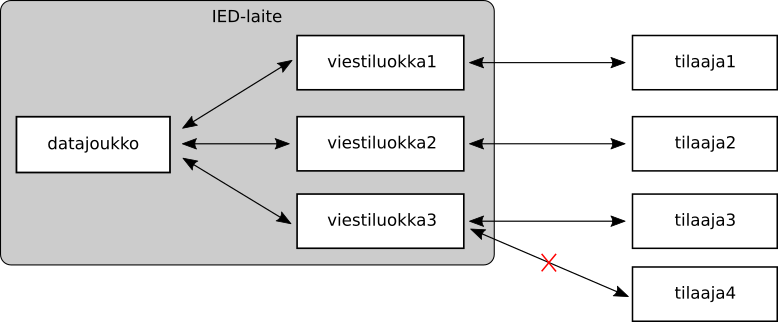
\includegraphics[width=1\textwidth]{pictures/rcbs-to-one-dataset.png}
	\caption{Kolme RCB-instanssia IED-laitteessa palvelee kolmea tilaajaa samasta datajoukosta.}
	\label{fig:rcb-to-one-dataset}
\end{figure}


\section{Viestien sisältö}
% Viestin sisältö koostuu yleisistä tiedoista ja taulukosta arvoja.
Tilaaja siis tilaa viestejä datajoukon muuttujien tapahtumista. RCB-instanssi puskuroi viestejä sille asetetun ajan ja kaikki tämän ajan sisällä tapahtuneet muuttujien tapahtumat sisällytetään samaan viestiin \cite[s.~98]{IEC61850-7-2}. Seurauksena on, että tilaajille lähetetyt viestit sisältävät taulukon arvoja, joka vaihtelee viestien välillä. Viestin siis koostuu yleisistä tiedoista ja taulukosta muuttujien arvoja \cite[s.~104]{IEC61850-7-2}. Viestin yleiset tiedot sisältävät kopioita RCB-instanssin muuttujista. Tämä toimii tietona tilaajalle millä arvoilla instanssi on konfiguroitu tilausta varten.

% Viestin vaihtoehtoiset kentät ja liipaisimet.
RCB-instanssi sallii tilaajan konfiguroida viestin kenttien määrää. Tilaaja voi poistaa viestistä tarpeetonta tietoa. Joitakin vaihtoehtoisia kenttiä ovat mm. syykoodit muuttujan sisältämiseen viestiin ja muuttujan viite arvon lisäksi. Tilaaja voi myös konfiguroida liipaisimia minkä tapahtumien pohjalta viesti lähetetään. \mbox{\cite[s.~90]{IEC61850-7-1}} \mbox{\cite[s.~98]{IEC61850-7-2}}

% Viesti pakataan biteiksi MMS-protokollan avulla.
Edellä esitetty viestin muoto on standardin mukainen abstrahoitu määritys. MMS-protokollan avulla viesti pakataan binäärimuotoon ja läheteään verkon yli tilaajalle. IEC 61850 standardin MMS-protokollan osa kertoo missä järjestyksessä bitit ovat \cite{IEC61850-8-1}. Tilaaja on vastuussa viestin purkamisesta standardin mukaisesti ymmärrettävään muotoon.


\section{Yhteenveto}
% Yhteenveto rajoitteista ja toiminnasta.
Standardin mukaisesti viestit tilataan IED-laitteelta julkaisija-tilaaja-paradigman mukaan. Tähän standardi ei tarjoa muita vaihtoehtoja. Viestit tilataan IED-laitteelta olevilta RCB-luokan instansseilta. Rajoituksena instanssille oli, että se voi palvella vain yhtä tilaaja kerrallaan ja instansseja IED-laitteessa on rajallinen määrä. Tämän lisäksi IED-laite voi rajoittaa yhteyksien määrää kiinteään lukuun, jonka jälkeen se hylkää loput yhteydenottopyynnöt. RCB-instanssit ja yhteyksien määrät konfiguroidaan IED-laitteelle käynnistyksen yhteydessä ja niitä ei voi muuttaa ajon aikana \cite{IEC61850-6}. Jos samaa datajoukkoa tarkkailee monta eri RCB-instanssia, lähetetään viestit IED-laitteessa tilaajille samasta tapahtumasta rinnakkain. Näitä tietoja tullaan myöhemmin käyttämään arkkitehtuurin ja ohjelmiston suunnittelussa.

% Käytetty kommunikointiprotokolla on MMS-protokolla.
Standardin abstrahoituja määrityksiä on mallinnettu eri tekniikoille. Tässä työssä kommunikointiin käytetään MMS-protokollaa, joka on TCP/IP-protokollaperheen päällä toimiva kommunikointiprotokolla. IED-laitteen kanssa kommunikoiva tilaajan täytyy purkaa binäärimuotoinen viesti ohjelmointikielen rakenteiksi. Diplomityössä toteutettu ohjelmisto käytti C-kielen \emph{libIEC61850}-kirjastoa kaiken MMS-kommunikoinnin toteuttamiseen \cite{libIEC61850-homepage}. Kirjasto tarjoaa korkean tason funktioita ja datarakenteita tiedon käsittelyyn ilman tietoa MMS-protokollan toiminnasta.
\chapter{Hajautettu järjestelmä}
\label{ch:distributed-systems}
% TODO: Kun tämän osion on kokonaan kirjoittanut niin siivoa tämä vastaamaan sitä.
Tässä osiossa käydään läpi järjestelmän hajauttamisen liityviä asioita, kuten mikä on hajautettu järjestelmä ja sen eri paradigmoja. Paradigmoista toteutetaan analyysi ja niistä arvioidaan niiden hyviä ja huonoja puolia. Lopuksi käsitellään avointa AMQP-standardia (engl. \emph{Advanced Message Queuing Protocol}) ja mitä hajautuksen paradigmoja se mahdollistaa.


\section{Mikä on hajautettu järjestelmä?}
\emph{Hajautettu järjestelmä} (engl. \emph{distributed system}) on verkko toisiinsa kytkettyjä fyysisiä- tai ohjelmistopohjaisia komponentteja, jotka kommunikoivat toistensa kanssa viestien välityksellä. Hajautetussa järjestelmässä osapuolten etäisyydellä ei ole merkitystä. Niiden välimatka voi olla eri maa tai sama rakennus. Hajautetut järjestelmät ovat oma tieteenala joka lähti liikkeelle käyttöjärjestelmien arkkitehtuurien tutkimuksista 1960-luvulla \cite[s.~384]{andrews2000foundations}. Ensimmäinen laajalle levinnyt hajautettu järjestelmä oli lähiverkot (engl. Local Area Network tai LAN), joka keksittiin 1970-luvulla \cite[s.~32]{andrews2000foundations}. Hajautetun järjestelmän määrityksistä ja toteuttamisesta on nykypäivänä olemassa hyvin kirjallisuutta ja tietoa, esimerkiksi \cite{distributed-systems-concepts-and-design, distributed-event-based-systems, mullender1993distributed, baldoni2005distributed}.

Järjestelmän hajautuksessa ja sen käytössä on pääasiassa kyse resurssien jakamisesta osapuolien kesken. Resurssi on abstrakti käsite ja voi tarkoittaa tekniikasta tai toteutuksesta riippuen montaa eri asiaa. Resurssilla voidaan esimerkiksi kuvata jaettua fyysistä laitetta kyten levyä tai tulostinta, ohjelmiston tapauksessa oliota tai tietokantaa \cite[s.~2--3]{distributed-systems-concepts-and-design}. Nykyinen internet mahdollistaa monien eri laitteiden kytkemisen verkkoon ja niiden kommunikoinnin keskenään, ja on nykypäivänä hyvä esimerkki todella laajasta hajautetusta järjestelmästä.

Hajautetussa järjestelmässä voidaan puhua osapuolten \emph{heterogeenisyydestä} (engl. \emph{heterogeneity}), eli osapuolet voivat kommunikoida toistensa kanssa tekniikasta tai toteutuksesta riippumatta. Tämä voidaan kuvata kerrosarkkitehruurin avulla. Korkean ja matalan tason ohjelmistojen välissä on ns. \emph{väliohjelmistokerros} (engl. \emph{middleware}). Tämän kerroksen tehtävä on abstrahoida matalan tason ohjelmisto tai alusta ja tehdä siitä heterogeeninen ylemmän tason ohjelmistoille ja palveluille. Kuvassa \ref{fig:middleware-architecture} on esitetty edelle mainittu kerrosarkkitehtuuri. \mbox{\cite[s. ~16--17]{distributed-systems-concepts-and-design}} \mbox{\cite[s.~2--3]{distributed-event-based-systems}}

\begin{figure}[ht!]
	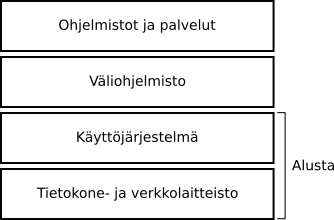
\includegraphics[width=0.5\textwidth]{pictures/middleware-architecture.png}
	\caption{Väliohjelmistokerros abstrahoimaan alusta heterogeeniseksi ylemmän tason ohjelmistolle (pohjautuu kuvaan \mbox{\cite[s.~52]{distributed-systems-concepts-and-design}}).}
	\label{fig:middleware-architecture}
\end{figure}


\subsection{Kuinka osapuolet kommunikoivat?}
Hajautetussa järjestelmässä osapuolet kommunikoivat keskenään viestien välityksellä. Jotta viestit voitaisiin vaihtaa tekniikasta riippumattomasti osapuolten välillä, täytyy tieto esittää alustariippumattomassa muodossa. Kommunikoivien osapuolten täytyy sopia yhteisestä viestin formaatista. Ohjelmat yleensä käsittelevät tietoa ohjelmistokielen tarjoamilla tietorakenteilla kuten esimerkiksi listoilla, puurakenteilla ja luokilla. Jotta tieto saadaan lähetettyä viestinä, täytyy se ensin muuntaa lähetykseen sopivaan muotoon. Tämä prosessi tunnetaan englannin kielellä nimellä \emph{marshalling}. Jotta vastaanotettua tietoa voidaa käyttää, täytyy viesti purkaa takaisin ohjelmistokielen rakenteiksi. Tämä prosessi englannin kielessä tunnetaan nimellä \emph{unmarshalling}. \mbox{\cite[s.~158]{distributed-systems-concepts-and-design}}

Kommunikointiin voidaan osapuolten välillä sopia erilaisista takuita lähetyksistä ja tiedon oikeudesta. Lähettäjä voi esimerkiksi vaatia vastaanottajaa kuittaamaan viestin vastaanottamisen. Jos kuittausta ei tule tietyn ajan sisällä, lähettäjä uudelleenlähettää viestin vastaanottajalle. Esimerkki tästä on TCP-protokollan (engl. Transmission Control Protocol) paketit, jossa lähettäjä odottaa vastaanottajan kuittausta paketista \cite[s.~9--10]{tcp-standard}. On myös tilanteita jossa lähettäjä ei välitä saako vastaanottaja viestin. Tässä tapauksessa osapuoli lähettää viestejä ilman tietoa siitä ottaako niitä kukaan vastaan. Esimerkki tästä on UDP-prokollan (User Datagram Protocol) paketit jossa lähettäjä ei odota kuittausta paketteihin \cite{udp-standard}. Uuden onnistuneesti lähetetyn paketin odotetaan korvaavan entisen tieto. Minkälainen takuu viestien lähetykseen valitaan riippu ohjelmiston vaatimuksista.


\subsection{Kommunikoinnin luokittelu}
Hajautetuissa järjestelmissä osapuolten kommunikoinnin välillä voi olla \emph{suora-} tai \emph{epäsuora liitos}. Suora liitos tarkoittaa tilannetta, jossa osapuolet tietävät toistensa identiteetin. Esimerkiksi lähettäjä lähettää viestiin suoraan vastaanottajalle. Epäsuora liitos tilannetta jossa osapuolet eivät tiedä toistensa identiteettiä. Epäsuorassa liitoksessa osapuolet yleensä kommunikoivat välittäjän kautta, joka hoitaa viestien lähettämisen toiselle osapuolelle. Suorassa liitoksessa toisen osapuolen vaihtaminen on vaikeampaa kuin epäsuorassa liitoksessa. Esimerkkinä tästä on yksinkertainen asiakas-palvelin-malli. Suoran liitoksen takia palvelin on vaikeampi vaihtaa toiseen samanlaiseen (palvelin tulkkaa HTML-sivuja asiakkalle). Epäsuorassa liitoksessa palvelimen vaihto samanlaiseen on helpompaa jos niiden välissä on tarpeeksi epäsuoruutta (geneerinen rajapinta tai välittäjä). \cite[s.~230]{distributed-systems-concepts-and-design}

Hajautetuissa järjestelmissä voidaan puhua erilaisista heikkojen liitoksien luokittelumalleista. Kirjallisuudessa näitä kutsutaan
\begin{itemize}
	\item \emph{heikko tilaliitos} (engl. \emph{space uncoupling}), tarkoittaa liitosta jossa osapuolet eivät tiedä toistensa identiteettiä, ja
	\item \emph{heikko aikaliitos} (engl. \emph{time uncoupling}), tarkoittaa liitosta jossa osapuolien ei tarvitse olla olemassa samaan aikaan.
\end{itemize}
Näiden mukaan voidaan esittää malli, jolla luokitellaan osapuolten välistä liitosta. Tämä malli on esitetty taulukossa \ref{tab:communication-models}. \cite[s.~230]{distributed-systems-concepts-and-design} \cite[s.~116]{eugster2003many}

\begin{table}[ht!]
	\caption{Hajautetussa järjestelmässä osapuolten kommunikoinnin luokittelun malli (pohjautuu taulukoihin \mbox{\cite[s.~231]{distributed-systems-concepts-and-design}} \mbox{\cite[s.~84]{cabri2000mobile}}).}
	\label{tab:communication-models}
	\begin{tabular}{p{0.1\linewidth} | p{0.37\linewidth} | p{0.37\linewidth}}
		\hline
		& \textbf{Vahva aikaliitos} & \textbf{Heikko aikaliitos} \\
		\hline
		\textbf{Vahva tilaliitos} & Kommunikointi tarkoitettu suoraan toiselle osapuolelle. Osapuolten täytyy olla olemassa samaan aikaan, esimerkiksi suora viestintä tai etäfunktiokutsu. & Kommunikointi tarkoitettu suoraan toiselle osapuolelle. Osapuolet voivat olla olemassa eri aikaan.\\
		\hline
		\textbf{Heikko tilaliitos} & Osapuolten ei tarvitse tietää toistensa identiteettiä. Osapuolten täytyy olla olemassa samaan aikaan, esimerkiksi IP-ryhmälähetys. & Osapuolten ei tarvitse tietää toistensa identiteettiä. Osapuolet voivat olla olemassa eri aikaan, esimerkiksi julkaisija-tilaaja ja viestijono \\
		\hline
	\end{tabular}
\end{table}

Taulukossa \ref{tab:communication-models} vasemmassa yläkulman luokittelu tarkoittaa kommunikointia, missä osapuolet tietävät toistensa identiteetin ja niiden täytyy olla olemassa samaan aikaan. Tämä on siis kaikista vahvin liitos mitä osapuolten välillä voi olla ja jossa on vähiten epäsuoruutta. Esimerkkinä tästä kommunikoinnista on etäfunktiokutsu tai suora viestintä prosesseiden välillä. Oikeassa yläkulmassa on tilanne, jossa osapuolet edelleen tietävät toistensa identiteetin, mutta niiden ei tarvitse olla olemassa samaan aikaan. Esimerkkinä osapuoli lähettää viestin tietylle identiteetille, mutta vastaanottaja ottaa viestin vastaan vasta myöhemmin. Teknistä esimerkkiä tähän tilanteeseen on hankalampi esittää kuin taulukon muihin kohtiin. Taulukon vasemmassa alakulmassa on tilanne jossa osapuolet eivät teidä toistensa identiteettiä, mutta niiden täytyy olla olemasa samaan aikaan. Esimerkkinä tästä on IP-ryhmälähetys, jossa viesti lähetetään kaikille verkon osapuolille ilman tietoa niiden identiteetistä. Vastaanottaja on olemassa samaan aikaan ja vastaa lähettäjälle ilman identiteettiä. Taulukon oikeassa alakulmassa on tilanne missä osapuolten välillä on kaikista eniten epäsuoruutta muista luokitteluista. Osapuolet eivät tiedä toistensa identiteettiä ja niiden ei tarvitse olla olemassa samaan aikaan. Esimerkkinä julkaisija-tilaaja- ja viestijono-paradigmat. \mbox{\cite[s.~230--232]{distributed-systems-concepts-and-design}} \mbox{\cite{cabri2000mobile}}

Epäsuoruus ohjelmoinnissa tuo hyötyjä ja joustavuutta ohjelmaan ja sen toimintaa kuten aikaisemmin tuotiin esille. Epäsuoruuden mukana tulee myös haittoja, kuten kommunikointi voi olla vaikeampaa osapuolten välillä ja epäsuoruus yleensä heikentää ohjelman suorituskykyä. Suorituskyky ja kommunikoinnin vaikeidet vaihtelevat tekniikasta ja toteutuksesta riippuen.

\section{Hajautuksen paradigmoja}
\begin{it}
	Lisätä tähän ongelmakohtaiset ja systeemikohtaiset osapuolet? Nyt on vain Ongelmakohtaiset osapuolet.
\end{it}
Hajautetussa järjestelmässä kommunikointi ja sen toteuttamisen mahdollisuudet ovat laajat ja vaihtoehtoja on paljon. Siksipä on tärkeää ymmärtää mitä ovat järjestelmän kommunikoivat osapuolet ja miten ne kommunikoivat. Näiden ymmärtäminen auttaa kehittäjää paremmin hahmottamaan vaihtoehtoja ja kokonaisuuden toimintaa.

Hajautetuissa järjestelmissä kommunikoivien osapuolien voidaan ajatella olevan \emph{olioita}, \emph{komponentteja} tai \emph{web-palveluita} (engl. \emph{World Wide Web}). Oliot tulevat suoraan olio-ohjelmoinnista ja on tarkoitettu jäsentämään asiaa tai toiminnallisuutta pienempiin omiin kokonaisuuksiinsa, joilla on oma sovittu rajapinta. Rajapinnan tarkoituksena on kapsuloida toiminnallisuutta helpokäyttöiseksi rajapinnaksi sen käyttäjälle. Komponenti on kokoelma olioita jotka muodostavat loogisen käytettävän kokonaisuuden. Komponenttit myös kommunikoivat rajapinnan läpi kuin oliot. Ero näiden välillä on, että komponentti oman rajapintansa lisäksi olettaa tiettyjä rajapintamäärityksiä muilta komponenteilta. Komponentti käyttää muiden komponenttien rajapintoja toteuttaaksen sille määritettyä toiminnallisuutta. Web-palvelut noudattavat samaa periaatetta rajapintojen kanssa kuin olio ja komponentti, mutta toimivat web-teknologioiden päällä. Olioita ja komponentteja käytetään toteuttamaan tiukemmin sidottuja ohjelmistoja. Web-palveluita käytetään toteuttamaan omia palvelukokonaisuuksia, joita voidaan liittää yhteen toteuttamaan kokonaisia applikaatioita. \mbox{\cite[s.~42--43]{distributed-systems-concepts-and-design}}

Hajautetussa järjestelmässä kommunikoinnin paradigmat voidaan jakaa kolmeen kategoriaan jotka on esitetty taulukossa \ref{tab:communication-paradigms}. Taulukossa tyyppien alla on esitetty sille tyypillisiä kommunikoinnin paradigmoja. Näitä paradigmoja käsitellään tarkemmin kappaleissa \ref{ch:interprocess-communication}, \ref{ch:remote-invocation} ja \ref{ch:indirect-communication}.

\begin{table}[ht!]
	\caption{Hajautetun järjestelmän kommunikointiparadigmat kolmella päätasolla (pohjautuu tauluun \mbox{\cite[s.~46]{distributed-systems-concepts-and-design}}).}
	\label{tab:communication-paradigms}
	\begin{tabular}{p{0.3\linewidth} | p{0.3\linewidth} | p{0.3\linewidth}}
		\hline
		\textbf{Prosessien välinen kommunikaatio} & \textbf{Etäkutsu} & \textbf{Epäsuora kommunikaatio} \\
		\hline \hline
		Viestien välitys (message passing) & Pyyntö-vastaus (request-reply) & Joukkokommunikointi (group communication) \\
		\hline
		Soketti (socket) & Etäproseduurikutsu (RPC) & Julkaisija-tilaaja (publish-subscribe) \\
		\hline
		Ryhmäkutsu (multicast) & Etämetodikutsu (RMI) & Viestijono (message queue) \\
		\hline
		& & Jonotaulu (tuple space) \\
		\hline
		& & Hajautetusti jaettu muisti (DSM) \\
		\hline
	\end{tabular}
\end{table}

\emph{Prosessien välinen kommunikointi} (engl. \emph{interprocess communication}) on matalan tason kommunikointia osapuolten välillä yleensä suoralla yhteydellä ohjelmointirajapintaan. \emph{Etäkutsut} (engl. \emph{remote invocation}) tarkoittavat toisen osapuolen kutsumista, joka suorittaa pyynnön ja palauttaa siihen vastauksen. Tyypillinen esimerkki tästä on asiakkaan pyyntö palvelimelle, johon palvelin lähettää takaisin vastauksen. Kahdessa aikaisemmin mainitussa kommunikoinnissa yhteistä on, että osapuolet tietävät eksplisiittisesti toistensa identiteetin ja niiden välillä on yleensä vahva aikaliitos. \emph{Epäsuora kommunikaatio} (engl. \emph{indirect communication}) tapahtuu kolmasta osapuolta käyttäen viestien välitykseen. Tämä mahdollistaa heikon liitoksen osapuolten välillä sekä ajallisesti että tilallisesti. Lähettäjä ei tiedä vastaanottajan identiteettiä ja toisin päin. Kolmas osapuoli vastaa viestin ohjaamisesta vastaanottajalle. \mbox{\cite[s.~43--45]{distributed-systems-concepts-and-design}}


\subsection{Prosessien välinen kommunikaatio}
\label{ch:interprocess-communication}
Prosessien välinen kommunikointi on matalan tason kommunikointia suoralla rajapinnan käytöllä. Esimerkkinä matalan tason kommunikoinnista on internet-protokollien käyttö, esimerkiksi UDP ja TCP. Käyttöjärjestelmät tarjoavat matalan tason rajapinnan kommunikointiin, esimerkiksi soketti-rajapinta. Soketti-rajapinnalla voidaan käyttää molempia UDP:tä ja TCP:tä \cite[s.~1152]{linux-programming-interface}. Tyypillistä tämän tason kommunikoinnille on että sen osapuolet tietävät toistensa identiteetin.

Käyttöjärjestelmän rajapintojen avulla prosessit voivat välittää viestejä suoraan toisilleen. Voidaan puhua, että prosessit lähettävät ja vastaanottavat toisilleen viestejä. Vastaanottaja toteuttaa yleensä jonon viestien vastaanottoon ennen käsittelyä. Jos kommunikointi on molemminsuuntaista, kummatkin osapuolet toteuttavat puskurin viestien vastaanottoon. Vastaanottaja voi kysellä tietoa jonosta toistuvasti saadakseen tiedon uudesta viestistä tai siitä voidaan keskeytyksellä. Viestien lähetys voi olla synkronista tai asynkronista. Synkronisessa viestien vaihdossa lähettäjä ja vastaanottaja sykronoidaan jokaisella viestillä. Eli viestin lähetys ja vastaanotto ovat pysäyttäviä (engl. blocking) operaatioita. Lähettäjän suoritus pysähtyy niin kauan kunnes vastaanottaja vastaa ja suoritus jatkuu. Asynkronisessa kommunikoinnissa operaatiot eivät ole pysäyttäviä (engl. non-blocking). Lähettäjä voi jatkaa muuta prosessointia heti kun viesti on kopioitu lähetyspuskuriin ja viestin lähetys jatkuu rinnakkain muun prosessoinnin kanssa. \mbox{\cite[s.~147--148]{distributed-systems-concepts-and-design}}

Hyviä puolia matalan tason kommunikoinnissa on, että sillä saadaan tehtyä saumaton kommunikointi prosessien välille ja sitä tukee moni nykyaikainen käyttöjärjestelmä. Matalan tason kommunikoinnin toteuttaminen vaatii paljon enemmän aikaa ja vaivaa ohjelmoijalta kuin korkeamman tason rajapinnan käyttö. Matalalla tasolla osapuolet ovat vahvasti liitoksissa ajallisesti ja tilallisesti. Osapuolet tietävät toistensa identiteetit ja niiden täytyy olla olemassa samaan aikaan. Vastaanottajan täytyy olla ottamassa vastaan viesti lähettäjältä samoihin aikoihin kun se lähetetään. Lisäksi matalantason ohjelma ei vältämättä ole modulaarinen ja on sidoksissa ympäristöönsä. Esimerkkinä Linux-käyt\-tö\-jär\-jes\-tel\-mäl\-le toteutettu ohjelma ei toimi Windows-käyttöjärjestelmällä. Tähän kuitenkin voidaan vaikuttaa ohjelman sisäisillä abstrahointitasoilla.


\subsection{Etäkutsu}
\label{ch:remote-invocation}
Etäkutsu paradigmoja ovat \emph{pyyntö-vastaus} (engl. \emph{request-reply}), \emph{etäproseduurikutsu} (engl. \emph{remote procedure call}, lyhennetään \emph{RPC}) ja \emph{etämetodikutsu} (engl. \emph{remote method invocation}, lyhennetään \emph{RMI}). Etäkutsuja voi suorittaa prosessit tai korkeamman tason objektit ja palvelut. Primitiivisin etäkutsu paradigmoista on pyyntö-vastaus, joka edustaa mallia aikaisemmin mainitun viestien välityksen päällä ja lisää siihen kaksisuuntaisen viestien vaihdon. Paradigmaa käytetään asiakas-palvelin kommunikoinnissa. \mbox{\cite[s.~185--186]{distributed-systems-concepts-and-design}}

Todella tärkeä määritys nykypäivän hajautettujen järjestelmien kannalta oli etäproseduurikutsut (RPC). Tämän määrittivät Birrell ja Nelson vuonna 1984 \cite{implemeting-remote-procedure-calls}. Se mahdollisti ohjelmoijan kutsua proseduuria toisella koneella etänä samoin kuin paikallista proseduuria. RPC-systeemi piilotti taustalle kaiken teknisen toteutuksen mitä kutsuun etänä tarvittiin, esimerkkinä tiedon siirron, pakkaamisen ja purkamisen \cite[s.~195--196]{distributed-systems-concepts-and-design}. Etämetodikutsu (RMI) toiminta on sama kuin RPC:n, mutta se on laajennettu toimivaksi olioilla. Olioiden metodeita voidaan kutsua niin kuin ne olisivat sen paikallisia metodeita \cite[s.~204]{distributed-systems-concepts-and-design}. Kummatkin RPC ja RMI tarjoavat saman tason abstraktion ohjelmoijalle ja piilottavat teknisen toteutuksen alleen.

Etäkutsuparadigmat ovat korkeamman tason paradigmoja kuin aikaisemmin mainittu prosessien välinen kommunikointi. Hyvänä puolena paradigmoissa on, että ohjelmoijan ei vältämättä tarvitse kirjoittaa matalan tason rajapinnan ohjelmaa. Rajapinta on abstrahoitu helppokäyttöisemmäksi ja sen toteutus ei vie niin paljon aikaa ja resursseja kuin matalan tason implementointi. Kuitenkin etäkutsut kärsivät samoista vahvoista liitoksista kuin prosessien väliset kutsut. Osapuolet ovat vahvasti liitoksissa ajallisesti sekä tilallisesti.


\subsection{Epäsuora kommunikaatio}
\label{ch:indirect-communication}
Epäsuora kommmunikaatio tarkoittaa osapuolten välistä kommunikaatiota välittäjän avulla. Osapuolet eivät vaihda tietoa suoraan keskenään ja eivät tiedä toisensa identiteettiä. Välittäjä huolehtii viestien reitittämisestä ja lähettämisestä vastaanottajalle. Välittäjän tarkempi toiminta ja tarkoitus vaihtelee toteutuksesta riippuen. Aikaisemmin mainittuissa kahdessa paradigmakategoriassa liitokset osapuolten välillä ovat pitkälti vahvoja ajallisesti sekä tilallisesti. Poikkeuksena tähän on esimerkiksi IP-ryhmälähetys, jossa osapuolilla on heikko tilaliitos, mutta vahva aikaliitos. Epäsuora kommunikointi osapuolten välillä vähentää liitoksien vahvuutta. Liitokset voivat olla heikkoja tilallisesti sekä ajallisesti ja niiden heikkous vaihtelee toteutuksesta riippuen. Epäsuora kommunikointi mahdollistaa toisen osapuolen helpomman vaihdon, siirron ja päivittämisen kuin suora kommunikointi. Useasti epäsuorassa kommunikoinnissa vastaanottajia voi olla monta yhden sijaan. Tällöin voidaan puhuta yksi-moneen-suhteesta (engl. one-to-many) osapuolten välillä. Epäsuoruus tuo hyötyjä, mutta se tuo myös väistämättöntä suorituskykykuormaa epäsuoruuden vaativan toiminnan takia. \mbox{\cite[s.~230--231]{distributed-systems-concepts-and-design}}

Epäsuoran kommunikoinnin paradigmoja ovat \emph{joukkokommunikointi} (engl. \emph{group communication}), \emph{julkaisija-tilaaja} (engl. \emph{publish-subscribe}), \emph{viestijono} (engl. \emph{message queue}), \emph{tuplesäilö} (engl. \emph{tuple space}) ja \emph{hajautetusti jaettu muisti} (engl. \emph{distributed shared memory}, lyhennetään \emph{DSM}). Nämä esitettiin aikaisemmin taulukossa \ref{tab:communication-paradigms}. Jokaista paradigmaa käsitellään erikseen tulevissa kappaleissa.

% TODO: Korjaa yllä oleva lause sitten kun on kirjoitettu loput kappaleet auki.


\subsection{Joukkokommunikointi}
Joukkokommunikointi on paradigma, jossa osapuoli lähettää viestin ryhmälle, jonka jälkeen viesti uudelleenlähetetään kaikille ryhmän osapuolille. Ryhmä vastaanottajia tunnistetaan yksilöivällä ryhmätunnisteella. Lähettäjä käyttää tunnistetta kohdentamaan viestin haluamalleen ryhmälle. Tässä tapauksessa lähettäjä ei ole tietoinen vastaanottajien identiteetistä \cite[s.~232--233]{distributed-systems-concepts-and-design}. Joukkokommunikointi tunnetaan myös \emph{joukkokommunikointisysteeminä} (engl. \emph{Group Communication System}, lyhennetään \emph{GCS}). Briman keksi ja kuvasi ensimmäinen tällainen systeemi 1986-luvulla \cite{isis-fault-tolerant-distributed-computing}. Joukkokommunikointi on tärkeä paradigma hajautettujen järjestelmien kannalta ja sillä on olemassa monta eri käyttökohdetta. Applikaatioina esimerkiksi voi olla kollaboraatio- ja monitorointi-ohjelmistot, jossa kaikkien osapuolien täytyy tietää uusimmasta muutoksesta.

Joukkokommunikoinnissa ryhmät voivat olla ns. avoimia tai suljettuja. Kuvassa \ref{fig:group-communication} on esitettu avoimen ja suljetun ryhmän toiminta. Avoin ryhmä mahdollistaa ulkopuolisen osapuolen lähettää viesti kaikille sen jäsenille. Suljettu ryhmä on tarkoitettu ainoastaan sen osapuolten väliseen kommunikointiin. Suljetussa ryhmässä yksi osapuoli voi ryhmälähettää viestin kaikille sen osapuolille ryhmän tunnisteella, samoin kuin ulkopuolinen avoimen ryhmän tapauksessa. Avoimen ja suljetun ryhmän lisäksi ryhmillä voi olla muitakin tärkeitä piirteitä. Ryhmät voivat olla päälekkäisiä tai ei päällekkäisiä. Päällekkäiset ryhmät mahdollistavat yhden osapuolen kuulua yhtä aikaa moneen ryhmään. Ei päälekkäisessä osapuoli voi kuulua enimmillään yhteen ryhmään. Joissakin tapauksissa ryhmän osapuolten voidaan sallia liittyä ja lähteä ryhmästä. Tällöin erillisen osapuolen täytyy pitää kirjaa ryhmän osapuolista ja tarjota toiminnallisuudet liittyä ja poistua ryhmästä. \mbox{\cite[s.~233--235]{distributed-systems-concepts-and-design}} \mbox{\cite[s.~48]{process-group-approach-briman}}

\begin{figure}[ht!]
	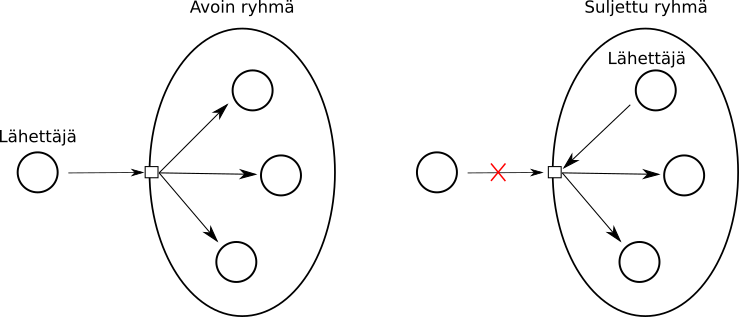
\includegraphics[width=1\textwidth]{pictures/group-communication.png}
	\caption{Osapuolten kommunikointi avoimessa ja suljetussa ryhmässä (pohjautuu kuvaan \mbox{\cite[s.~235]{distributed-systems-concepts-and-design}}).}
	\label{fig:group-communication}
\end{figure}

Ryhmät mahdollistavat yhden-moneen-suhteen kommunikoinnissa. Yksi viesti saadaan lähetettyä monelle osapuolelle yhdeltä kertaa. Tämä säästää kaistaa verrattuna tilanteeseen, jossa viesti lähetettäisiin jokaiselle osapuolelle erikseen. Joukkokommunikoinnissa osapuolten välillä on heikko tilaliitos, mutta vahha aikaliitos. Joukkokommunikointisysteemit ovat monimutkaisia ja niiden lähetystakuiden vaatimukset vaativat paljon vaivannäköä systeemiltä. Lähetystakuihin yleensä kuuluu että jokainen ryhmän jäsen saa sille lähetetyn viestin ainakin kerran jossakin vaiheessa. Dynaamisen ryhmän tapauksessa, jossa osapuolia voi tulle ja lähteä ryhmästä, lähetystakuiden kiinni pitäminen monimutkaistuu entisestään. \mbox{\cite{group-communication-specification}} \mbox{\cite[s.~236]{distributed-systems-concepts-and-design}}


\subsection{Julkaisija-tilaaja}
Julkaisija-tilaaja on kommunikointiparadigma, jossa \emph{julkaisijat} julkaisevat tapahtumia/viestejä ja \emph{tilaajat} tilaavat halumiaan tapahtumia/viestejä \emph{tilauksilla}. Osapuolten välissä on julkaisija-tilaaja-systeemi, joka vastaa viestien reitittämisestä tilaajille tehtyjen tilauksien perusteella. Järjestelmä mahdollistaa monen tilaajan tilata viestejä samalta julkaisijalta. Näin ollen kommunikointisuhde osapuolten välissä on yksi-moneen, kuten joukkokommunikoinnissa. Systeemiin tehdyllä tilauksella tilaaja voi tilata samalla kertaa monta eri julkaisijaa. Tehty tilaus on ns. \emph{suodatin/malli} (engl. \emph{pattern}), joka systeemin sääntöjen mukaan voi täsmätä enemmän kuin yhteen julkaistuun viestiin. Kirjallisuudessa paradigma tunnetaan nimellä \emph{julkaisija-tilaaja-systeemi} (engl. \emph{publish-subscribe system}) \cite{baldoni2005distributed}, sekä \emph{hajautettu tapahtumapohjainen systeemi} (engl. \emph{distributed event-based system}) \cite{distributed-event-based-systems}. Julkaisija-tilaaja-paradigmalle on olemassa monia erilaisia käyttökohteita hajautetuissa järjestelmissä. Varsinkin systeemeissä, jossa erilaisten tapahtumien ja viestien jakaminen eri osapuolille on tarpeen. IEC 61850 -standardissa käsitelty viestien tilaus IED-laitteelta käyttää juuri tätä kommunikointiparadigmaa.

Julkaisija-tilaaja-systeemin voidaan ajatella tarjoavan funktioita, joita osapuolet käyttävät toimiakseen sen kanssa. Kuvassa \ref{fig:publish-subscribe-communication} on esitetty systeemin toiminta näitä funktioita käyttäen. Julkaisija julkaisee viestin systeemiin funktiolla \emph{julkaise(v)}, jossa parametri v kuvaa julkaistavaa viestiä. Tilaaja tilaa viestejä funktiolla \emph{tilaa(s)}, jossa s-parametri tarkoittaa suodatinta viesteihin joihin tilaaja osoittaa kiinnostusta. Viestin saapuessa systeemiin ja tilauksen suodattimen täsmätessä, viesti lähetetään tilaajalle \emph{ilmoita(v)} funktiolla, jossa v on julkaistu viesti. Tilaajien on myös mahdollista peruuttaa tilaus \emph{peruuta\_tilaus()} funktiolla. Joissakin systeemeissä julkaisijoiden on myös mahdollista mainostaa viestejä. Julkaisija kutsuu \emph{mainosta(s)} funktiota, jossa s-parametri kertoo viestien tyypistä ja noudattaa samaa formaattia kuin tilaajien suodattimet. Mainostus voidaan perua \emph{peruuta\_mainos()} funktiolla. \mbox{\cite[s.~2--3]{baldoni2005distributed}} \mbox{\cite[s.~26--28]{distributed-event-based-systems}}

\begin{figure}[ht!]
	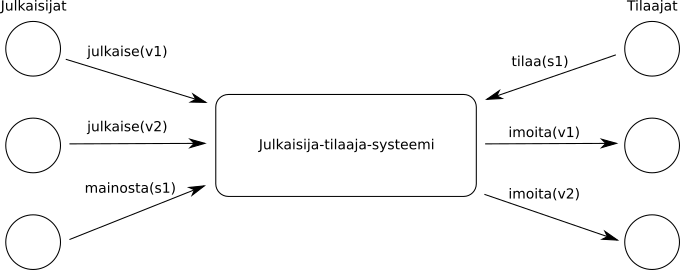
\includegraphics[width=0.9\textwidth]{pictures/publish-subscribe.png}
	\caption{Julkaisija-tilaaja-systeemi välikätenä viestien välittämisessä julkaisijoiden ja tilaajien välissä (pohjautuu kuvaan \mbox{\cite[s.~246]{distributed-systems-concepts-and-design}}).}
	\label{fig:publish-subscribe-communication}
\end{figure}

Julkaisija-tilaaja-systeemin ansiosta kommunikointi osapuolten välillä on epäsuoraa. Kommunikoinnissa osapuolten välillä on heikko tilaliitos ja vahva aikaliitos. Heikkossa tilaliitoksessa osapuolet eivät tiedä toistensa identiteettiä kuka julkaisi viestin ja kuka sen vastaanottaa. Systeemi osapuolten välissä mahdollistaa tämän. Osapuolten välillä on kuitenkin vahva aikaliitos. Jotta tilaaja saa viestin, täytyy sen olla olemassa samaan aikaan kuin julkaisijan. Yksinkertaisin julkaisija-tilaaja-systeemi on helppo implementoida yhdellä välittäjällä. Tämä voi kuitenkin tulla ongelmaksi tai pullonkaulaksi järjestelmässä, missä tiedon vaihto on nopeaa ja osapuolia on paljon tai välittäjä kaatuu kesken kaiken. Tällaisen systeemin skaalaaminen ylöspäin on vaikempaa ja vaatii hajautettua välittäjäverkkoa \cite[s.~248--249]{distributed-systems-concepts-and-design}. Lisäksi systeemin epäsuoruus tuo mukanaan kommunikointiin vaikeutta ja suoritukseen kuormaa verrattuna suoraan kommunikointiin.


\subsection{Viestijono}
Viestijono paradigmassa osapuolet kommunikoivat epäsuorasti jonon välityksellä. Joukkokommunikointi ja julkaisija-tilaaja paradigmat ovat yksi-moneen-suhde osapuolten välillä, kun taas viestijono on yksi-yhteen-suhde (engl. point-to-point). Lähettäjä lähettää viestin jonoon, josta vastaanottaja poistaa sen käsittelyyn. Viestijonon tarkoitus on puskuroida viestejä vastaanottajalle ja näin taata niiden saatavuus ja järjestys millä ajan hetkellä hyvänsä. Viestijono mahdollistaa siis osapuolten välillä heikon tila- ja aikaliitoksen. Jonon ansiosta lähettäjä ja vastaanottaja voivat olla olemassa eri aikaan \cite[s.~254]{distributed-systems-concepts-and-design}. Kuvassa \ref{fig:message-queue-communication} on esitetty viestijonosysteemin toiminta osapuolten välillä.

\begin{figure}[ht!]
	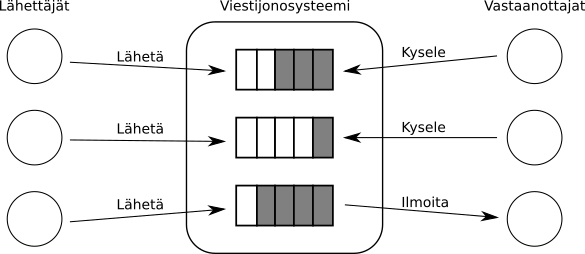
\includegraphics[width=0.9\textwidth]{pictures/message-queue.png}
	\caption{Viestijonosysteemi puskuroi viestejä lähettäjiltä vastaanottajille (pohjautuu kuvaan \mbox{\cite[s.~255]{distributed-systems-concepts-and-design}}).}
	\label{fig:message-queue-communication}
\end{figure}

Vastaanottaja voi poistaa viestejä jonosta kolmella eri periaatteella:
\begin{itemize}
	\item \emph{pysäyttävä vastaanotto} (engl. \emph{blocking receive}), joka pysäyttää kunnes viesti on saatavissa,
	\item \emph{ei pysäyttävä vastaanotto} (engl. \emph{non-blocking receive}), joka tarkistaa jonon tilan ja palauttaa viestin jos saatavilla, ja
	\item \emph{ilmoita} (engl. \emph{notify}), joka lähettää tiedon uudesta viestistä kun sellainen on saatavilla \cite[s.~254]{distributed-systems-concepts-and-design}.
\end{itemize}
Ei pysäyttävä vastaanotto on sama kuin vastaanottaja kyselisi viestejä jonosta tietyn väliajoin (engl. poll). Viestijonosysteemissä jonoa ei ole rajoitettu yhteen lähettäjään ja vastaanottajaan. Systeemissä moni lähettäjä voi lähettää viestejä samaan jonoon ja moni vastaanottaja voi vastaanottaa niitä samasta jonosta. Jonojen jonotuspolitiikka on yleensä FIFO-periaate (engl. First-In-First-Out). Moni systeemi kuitenkin tukee myös muitakin periaatteita, kuten viestien priorisointia, jossa ylemmän prioriteetin viestit käsitellään ennen alemman prioriteetin viestejä \cite[s.~120]{eugster2003many}.

Viestijonon hyvänä puolena on osapuolten heikon aikaliitoksen mahdollistaminen. Tämä mahdollistetaan sillä, että viestit jonossa ovat pysyviä (engl. persistent). Systeemi tallentaa viestit levylle, jossa ne säilyvät niin kauan kunnes vastaanottaja poistaa ne jonosta. Systeemi takaa viestien lähettämisen vastaanottajalle. Viesti tullaan lähettämään jossakin vaiheessa ja enintään kerran. Lisäksi lähetetty viesti vastaa alkuperäistä lähettäjän viestiä. \mbox{\cite[s.~255]{distributed-systems-concepts-and-design}}

Aikaisemmin käsiteltiin viestien välitystä prosessien välisessä kommunikoinnissa ja mainittiin että prosessit voivat implementoida jonon viestien vastaanottoon. Jonosysteemillä on paljon samanlaisia piirteitä tämän kanssa. Kuitenkin viestien välityksessä jonot ovat liitoksissa sen osapuoleen ja ovat implisiittisiä. Viestijonosysteemissä jonot ovat kolmannen osapuolen tarjoamia eksplisiittisiä jonoja, joka erottaa lähettäjät ja vastaanottajat toisistaan. Tämä on tärkeä ero, joka tekee viestijonosta oman epäsuoran kommunikointiparadigman. \mbox{\cite[s.~256]{distributed-systems-concepts-and-design}}

% TODO: Kirjoita tähän vielä muista jos tarpeen? (jaettu muisti, tuple space)
\chapter{Järjestelmän suunnittelu}
\label{ch:architecture-planning}
% Tuttuja asioita: hajautetun järjestelmän teoria ja sen paradigmat, IEC 61580 -standardin pääpiirteinen toiminta ja sen rajoitteet.
% Diplomityön prosessin pääpiirteinen kuvaus suunnittelusta toteutukseen.
Diplomityön suunnittelu aloitetaan ensin hajautetun järjestelmän arkkitehtuurin suunnittelusta. Tässä luvussa arkkitehtuuri suunnitellaan analysoimalla aikaisemmin läpikäytyjä hajautetun järjestelmän paradigmoja ja IEC 61850 -standardin asettamia määrityksiä. Tuloksena on arkkitehtuurisuunnitelma osaksi muuta järjestelmää, joka määrittää kommunikointiparadigmat viestien kuljettamiseen IED-laitteilta järjestelmän muille komponenteille. Tulevissa luvuissa tätä suunnitelmaa tullaan tarkentamaan toteutukseen käytettävillä tekniikoilla, joka työn lopussa toteutetaan ohjelmistoksi.


\section{Arkkitehtuurin analyysi}
\label{ch:architecture-analysis}
IEC 61850 -standardi määrittää, että viestit IED-laitteelta tulevat julkaisija-tilaaja-pa\-ra\-dig\-man mukaisesti. Viestit tilataan IED-laitteelta olevilta RCB-luokkien instansseilta. RCB-instanssi on kytketty laitteella olevaan datajoukkoon, jonka tiedoista ollaan kiinnostuneita. Rajoituksena standardi asetti, että tilaajan täytyy varata RCB-instanssi ja yksi RCB-instanssi voi palvella vain yhtä tilaajaa kerrallaan. RCB-instansseja IED-laitteissa on rajallinen määrä yhtä datajoukkoa kohti ja näitä voidaan myös käyttää aseman sisäiseen toimintaan. Tässä työssä käsitellyssä IED-laitteessa yhteen datajoukkoon oli esimerkiksi määritetty viisi eri RCB-instanssia. Seurauksena on, että kyseisen datajoukon voi tilata vain viisi saman aikaista tilaajaa. Lisäksi tässä työssä testattu IED-laite rajoitti avoimet yhteydet viiteen. Tästä ylimeneviä yhteyksiä ei avattu, ja IED-laite palautti standardin mukaisen negatiivisen vastauksen.

Vaatimus V2 määritti, että IED-laitteen tilatut viestit täytyy saada jaettua järjestelmän muiden komponenttien kanssa. Työn tekohetkellä komponentteja järjestelmässä oli kaksi: mittaustiedon näyttämiseen ja tilatiedon tarkkailuun. Vaatimus V3 määritti, että komponenttien määrän pitää pystyä muuttumaan järjestelmän tarpeiden mukaan. Tämä vaatimus asetettiin tulevaisuuden varalle, jolloin komponentteja on mahdollisesti enemmän kuin kaksi.

Edelle mainituista IED-laitteen rajoituksista ja työlle asetetuista vaatimuksista voidaan tehdä johtopäätöksiä hajautuksen arkkitehtuurin suhteen. Samalle IED-laitteelle avattujen yhteyksien määrä halutaan pitää pienenä. Tämän lisäksi varattujen RCB-instanssien määrä jokaista datajoukkoa kohti halutaan myös pitää pienenä. Edellä mainittujen perusteella aseman resursseja halutaan varata mahdollisimman vähän ja vapauttaa niitä aseman muuhun toimintaa. Lisäksi vaaditut resurssit pitää pystyä määrittämään ennalta. Tämä helpottaa aseman insinöörin suunnittelutyötä, koska hän voi ottaa luvut huomioon IED-laitteiden konfiguroinnissa.

Edellä mainittuun tilanteeseen ratkaisuna olisi ollut, että järjestelmän yksittäiset komponentit tilaisivat niiden tarvitsemat tiedot suoraan IED-laitteelta. Tämä on esitetty kuvan \ref{fig:architecture-analysis} yläosassa. Ongelmana tässä kuitenkin on aikaisemmin mainittu yhteyksien määrän rajoitus IED-laitteelle ja se, että niiden määrä haluttiin minimoida ja pitää vakiona. Lisäksi viestit tilataan ja palautetaan komponentille MMS-protokollamäärityksien mukaisesti. Seurauksena on, että jokainen komponentti joutuu käsittelemään MMS-protokollan binääridataa itse tai kirjaston avulla. Viestin muoto olisi parempi olla ymmärrettävämpi. Näin viestin lukeminen eri tekniikoilla olisi helpompaa. Tämän asetti vaatimus V8 ja oli myös T3 tutkimuskysymyksen aihe.

\begin{figure}[ht!]
	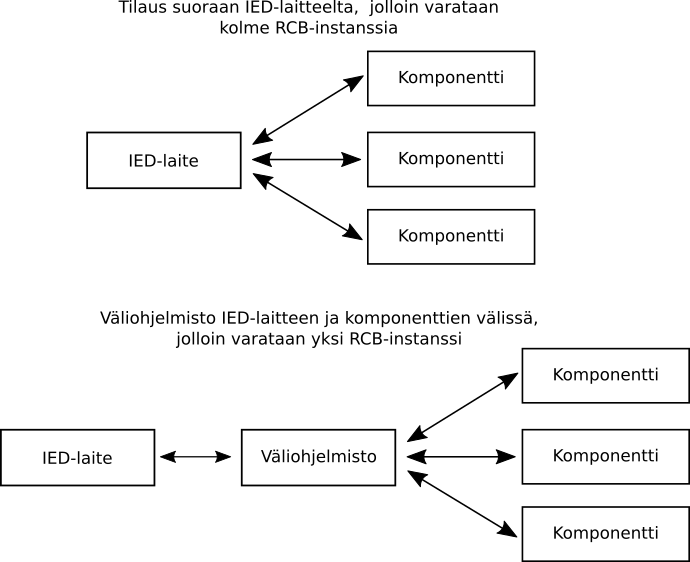
\includegraphics[width=0.7\textwidth]{pictures/architecture-analysis.png}
	\caption{IED-laitteelta viestien tilaus suoraan ja väliohjelmiston avulla.}
	\label{fig:architecture-analysis}
\end{figure}

Ratkaisuna edellä mainittuun tilanteeseen on kommunikoinnin epäsuoruuden lisääminen. Epäsuoruutta saadaan aikaan toteuttamalla erillinen ohjelmistokomponentti IED-laitteen ja muiden järjestelmän komponenttien väliin. Tätä komponenttia voisi kutsua myös nimellä \emph{väliohjelmisto} (\emph{middleware}) ja on esitetty kuvan \ref{fig:architecture-analysis} alaosassa. Väliohjelmisto tilaisi viestit IED-laitteelta ja halutuilta RCB-instansseilta. Samalla komponentti muokkaisi saapuvat viestit parempaan muotoon, joka olisi helpompi muiden järjestelmän komponenttien lukea. Väliohjelmiston avulla yhteyksien määrä IED-laitetta kohti saadaan yhteen. Tämän avulla myös saadaan minimoitua varattujen RCB-instanssien määrä datajoukkoa kohti yhteen. Tuloksena on vakiomäärät yhteyksiä ja RCB-instansseja datajoukkoa kohti, jotka ovat helpompi ennustaa ja konfiguroida etukäteen tarpeiden mukaan.

Vaatimuksessa V4 mainittiin myös, että muu järjestelmä ohjaa viestien tilauksen aloittamista ja lopettamista. Väliohjelmistoa on mahdollista muun järjestelmän ohjata tilauksien mukaan. Väliohjelmisto ja epäsuoruus myös helpottavat viestien puskuroinnin toteuttamista komponenteille, joka oli vaatimus V6. Ilman epäsuoruutta, jokaisen komponentin tulee toteuttaa oma sisäinen puskuri viestien vastaanottamiseen.

Tässä kappaleessa analysoitiin IEC 61850 -standardin asettamia rajoja ja ohjelmistolle asetettuja vaatimuksia. Näistä analysoitiin mikä olisi toimiva ratkaisu tässä tilanteessa järjestelmän hajauttamiseen korkealla tasolla. Tuloksena järjestelmään päätettiin lisätä epäsuoruutta toteuttamalla väliohjelmisto IED-laitteen ja järjestelmän muiden komponenttien väliin. Jäljelle jää vielä miettiä vastaukset seuraaviin kysymyksiin:
\begin{itemize}
	\item Mitkä kommunikointiparadigmat toteuttavat väliohjelmiston ja komponenttien vaatimukset?
	\item Mihin muotoon matalan tason MMS-viesti väliohjelmistossa tulee muuntaa jakoa varten?
	\item Mitkä ovat väliohjelmiston ja muiden komponenttien välisten liitoksien vahvuudet?
	\item Kuinka viestien puskurointi väliohjelmiston avulla toteutetaan?
\end{itemize}


\section{Osapuolten liitoksien analyysi}
Aikaisemmin kappaleessa \ref{ch:liitokset} käsiteltiin hajautetun järjestelmän osapuolten välisiä liitoksia. Erilaisten liitoksien luokittelut esiteltiin taulukossa \ref{tab:communication-models}. Lisäksi hajautetussa järjestelmässä kommunikointi osapuolten välillä voi olla suoraa tai epäsuoraa. Aikaisemmin kohdassa \ref{ch:architecture-analysis} päädyttiin lisäämään epäsuoruutta IED-laitteen ja järjestelmän muiden komponenttien väliin.

IED-laitteen ja viestien tilaajan välinen kommunikointi on suoraa ja se ei tapahdu välittäjän kautta. Lisäksi osapuolten välillä on vahva väli- ja aikaliitos. Kommunikoinnissa osapuolet tietävät toistensa identiteetin (IP-osoitteen), jonka seurauksena niiden välillä on vahva väliliitos. Kommunikoinnissa on myös vahva aikaliitos, koska osapuolien täytyy olla olemassa samaan aikaan. Tilaajan täytyy olla ottamassa viesti vastaan, kun IED-laite sen lähettää ja IED-laitteen pitää olla olemassa, kun tilaus tehdään. Kaikki edellä mainitut tulevat IEC 61850 -standardin määrityksien seurauksena ja näihin ei työssä voida vaikuttaa.

Työn aloitushetkellä järjestelmässä oli kaksi tietoa tarvitsevaa komponenttia. Lisäksi vaatimus V3 asetti, että näiden komponenttien määrä voi muuttua tarpeiden mukaan. Näistä seurauksena väliohjelmiston ja muiden järjestelmän komponenttien välinen suhde on yksi-moneen. Toteuttamalla suora kommunikointi väliohjelmiston ja järjestelmän muiden komponenttien väliin, väliohjelmiston täytyy tietää muiden komponenttien olemassaolosta ja kenelle viestit ohjataan. Tämä lisäisi osapuolten välistä riippuvuutta ja vähentäisi toteutuksen joustavuutta. Ratkaisuna on lisätä epäsuoruutta väliohjelmiston ja muiden komponenttien väliin välittäjällä. Tämä on esitetty kuvassa \ref{fig:coupling-analysis}. Välittäjä vähentää osapuolten välistä riippuvuutta ja lisää toteutuksen joustavuutta. Se myös auttaa toteuttamaan asetettuja vaatimuksia, kuten viestien puskurointia (V6) ja uuden viestin ilmoitusta (V5). Vaatimus V7 asetti, että komponenttien pitää pystyä suodattamaan tietoa sen lähteen perusteella. Välittäjän tuoma epäsuoruus auttaa myös tämän vaatimuksen toteuttamisessa. Tällä vastuu väliohjelmistolta viestien jakamisesta saadaan siirrettyä välittäjän vastuulle.

\begin{figure}[ht!]
	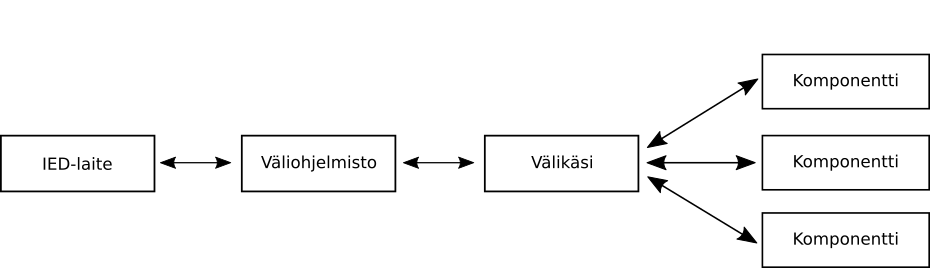
\includegraphics[width=1\textwidth]{pictures/coupling-analysis.png}
	\caption{Välittäjä väliohjelmiston ja komponenttien välissä lisäämään epäsuoruutta ja joustavuutta.}
	\label{fig:coupling-analysis}
\end{figure}

Väliohjelmiston ja muiden komponenttien välille edellä mainitun perusteella halutaan heikko väliliitos. Väliohjelmiston ei tarvitse tietää järjestelmän muiden komponenttien identiteettiä ja tämä parantaa toteutuksen joustavuutta. Aikaliitos asetettujen vaatimuksien perusteella pystyisi olemaan vahva tai heikko. Kuitenkin muu järjestelmä ohjaa tilauksen aloittamista ja lopettamista (vaatimus V4). Seurauksena on, että väliohjelmisto ja muut komponentit ovat olemassa samaan aikaan. Tämä poistaa tarpeen heikolle aikaliitokselle.

Tässä kappaleessa analysoitiin hajautetussa järjestelmässä olevien osapuolien liitoksien vahvuutta. IEC 61850 -standardi asettaa rajoitteet IED-laitteen ja väliohjelmiston välille, joihin ei voida vaikuttaa. Väliohjelmiston ja muiden komponenttien väliin päädyttiin toteuttamaan epäsuora kommunikointi joustavuuden ja vaatimusten takia. Samojen osapuolten väliin halutiin toteuttaa heikko väliliitos ja vahva aikaliitos. Kysymyksenä jää miettiä millä hajautuksen paradigmoilla välittäjä tulee toteuttaa, jotta saadaan halutut ominaisuudet?


\section{Paradigmojen analyysi}
Aikaisemmissa kappaleissa analyysien ja vaatimusten pohjalta päädyttiin kuvan \ref{fig:coupling-analysis} hajautetun järjestelmän arkkitehtuuriin. Tässä kappaleessa vertaillaan ja analysoidaan eri hajautuksen paradigmoja. Tarkoituksena on selvittää mitä paradigmoja tarvitaan, jotta asetetut vaatimukset voidaan toteuttaa. Näitä olivat viestien puskurointi (V6), ilmoitukset komponenteille uuden viestin saapuessa (V5) ja viestien suodattamisen mahdollisuus IED-laitteen mukaan (V7). Tässä kappaleessa käsitellyt paradigmat koskevat kuvan \ref{fig:coupling-analysis} välittäjää väliohjelmiston ja järjestelmän komponenttien välissä. Hajautetun järjestelmän eri paradigmat oli esitetty taulukossa \ref{tab:communication-paradigms}.

Järjestelmään haluttiin epäsuoruutta välittäjällä. Tätä parhaiten tarjoavat epäsuorat kommunikointiparadigmat. Vaatimus V6 määritti, että viestejä pitää pystyä puskuroimaan myöhempään ajan hetkeen, jos komponentti ei niitä ehdi käsitellä. Tämän ominaisuuden parhaiten tarjoaa viestijonoparadigma. Viestejä haluttiin erotella IED-laitteen mukaan (V7), ja komponentit voisivat päättää itse mistä ovat kiinnostuneita. Tätä ominaisuutta epäsuorista paradigmoista tarjoavat joukkokommunikointi ja julkaisija-tilaaja. Joukkokommunikoinnissa komponentti pystyisi olemaan osa haluttuja ryhmiä. Julkaisija-tilaaja-paradigmassa komponentti pystyisi tilaamaan halutut viestit. Kummatkin edellä mainituista tarjoavat myös halutut ilmoitukset (V5). Joukkokommunikointi- ja julkaisija-tilaaja-systeemissä vastaanottajat saavat ilmoituksen uuden viestin saapuessa. Jotta joukkokommunikoinnilla saadaan haluttu toiminnallisuus, tulee ryhmän olla avoin ja sen pitää mahdollistaa osapuolten liittyminen ja poistuminen ryhmästä. Lisäksi ryhmien pitää sallia olevan päällekkäisiä. Tämä sen takia, että komponentin on mahdollisesti saada viestejä useammasta lähteestä samaan aikaan.

Järjestelmään halutun epäsuoruuden takia suorat kommunikointiparadigmat eivät sovellu kovin hyvin hajautuksen toteuttamiseen. Näitä olivat prosessien välinen kommunikointi ja etäkutsut. Hajautuksessa osapuolien välillä haluttiin olevan heikko väliliitos ja vahva aikaliitos. Kummassakin edellä mainitussa paradigmassa liitokset ovat vahvoja. Suoralla kommunikoinnilla vastaanottavan osapuolen pitää toteuttaa viestipuskuri itse, verrattuna jos käytettävä epäsuora systeemi tarjoaisi puskurin sen sijaan. Tämä hankaloittaa uusien komponenttien kehitystyötä. Muu järjestelmä on toteutettu web-sovelluksena, josta seurasi vaatimus V10, että kommunikoinnin pitää toimia TCP/IP-protokollaperheen päällä. Prosessien välinen kommunikointi tapahtuu mm. pistokkeilla ja näin ollen on vaatimukseen nähden liian matalaa. Etäkutsut tarjoavat tähän paremman vaihtoehdon, mutta vaatimuksissa ei ollut tarvetta pyyntö-vastaus-kommunikoinnille. Viestien suunta on tässä tapauksessa yhden suuntaista IED-laitteelta järjestelmän komponentille.

Asetettuihin vaatimuksiin nähden epäsuorat paradigmat sopivat toteutukseen parhaiten. Näistä tarvitaan viestijonoparadigmaa viestien puskurointiin ja joukkokommunikointi tai julkaisija-tilaaja niiden lähettämiseen komponenteille. Joukkokommunikointi ja julkaisija-tilaaja paradigmat ovat kummatkin tilanteeseen sopivia vaihtoehtoja. Vielä pitää miettiä millä tekniikalla halutut paradigmat toteutetaan. Valitun tekniikan tulee yhdistää kaksi eri paradigmaa niin, että viestien oikea reitittäminen ja puskurointi ovat mahdollisia.

% TODO: Miettiä onko muita syitä hylätä joukkokommunikointi vaihtoehtona kuin tekniikan valinta.


\section{Toteutustekniikoiden vertailu}
Hajautetun järjestelmän toteuttamiseen löytyy erilaisia avoimia standardeja kuten \emph{AMQP} (\emph{Advanced Message Queuing Protocol}) \cite{amqp-homepage} ja \emph{MQTT} (\emph{Message Queuing Telemetry Transport}) \cite{mqtt-homepage}. Standardien tarkoitus on määrittää yhteiset säännöt osapuolten kommunikointiin hajautetussa järjestelmässä. Standardien pohjalta on toteutettu erilaisia viestien välitysohjelmistoja, joihin muut osapuolet voivat ottaa yhteyttä standardin mukaisesti tekniikasta riippumatta. Kummatkin edellä mainitut standardit ovat määritetty toimivaksi TCP/IP-protokollaperheen päällä \cite[s.~1]{mqtt-specification} \cite[s.~22]{AMQP-specification}.

MQTT on julkaisija-tilaaja-paradigmaan pohjautuva kommunikointistandardi. MQTT""-""mää\-ri\-tyk\-si\-en mukainen välittäjäpalvelin tarjoaa myös viestien puskuroinnin mahdollisuuden \cite{mqtt-specification}. MQTT on pääasiassa tarkoitettu kommunikointiin, missä kaista on rajallista ja kommunikoinnista huolehtivan koodin jalanjälki pitää olla pientä. Tästä syystä se on paljon käytetty standardi IoT-laitteissa (Internet of Things) ja kotiautomaatiossa \cite[s.~9--11]{mqtt-for-iot}.

AMQP-standardi on tarkoitettu \emph{MOM}:in toteuttamiseen (\emph{Message-Oriented Middleware}) ja näin ollen mahdollistaa monen eri kommunikointiparadigman toteuttamisen \cite[s.~6]{AMQP-specification}. MOM tarkoittaa hajautetussa järjestelmässä \emph{väliohjelmistoa} (\emph{middleware}), jota käytetään lähettämään ja vastaanottamaan viestejä. MOM:in tarkoitus on tarjota heterogeeninen alusta viestien vaihtoon tekniikasta ja verkkoprotokollasta riippumatta \cite{mom}. AMQP-standardi mahdollistaa esimerkiksi viestijonot, etäkutsut ja erilaiset reititykset kuten pisteestä pisteeseen ja julkaisija-tilaaja. AMQP tarjoaa toteutukseen enemmän paradigma vaihtoehtoja kuin MQTT.

Tässä työssä toteutuksen tekniikaksi valittiin AMQP. AMQP tarjoaa kaikki vaaditut ominaisuudet välittäjän toteuttamiseen. AMQP ei mahdollista joukkokommunikoinnin toteuttamista, mutta mahdollistaa julkaisija-tilaaja-paradigman. Aikaisemmin julkaisija-ti\-laa\-ja-paradigma todettiin toteutukseen sopivaksi vaihtoehdoksi joukkokommunikoinnin kanssa. AMQP tarjoaa viestien puskuroinnin jokaista tilaajaa kohden ja komponenttien on mahdollista myös suodattaa viestejä kiinnostuksen mukaan. MQTT olisi myös todennäköisesti sopinut toteutukseen, koska se tarjosi kaikki vaaditut ominaisuudet. Työssä kuitenkin päädyttiin AMQP:n valintaan tekijän aikaisemman kokemuksen ja muiden työntekijöiden kanssa käydyn keskustelun tuloksena. Viestien lähetykselle järjestelmässä ei vaadittu takuita, mutta nämä olisi hyvä olla olemassa tulevaisuuden takia (V11). AMQP tarjoaa takuumekanismit viestien lähettämiseen transaktioina ja vastaanottamiseen niiden kuittaamisella \cite[s.~14,21]{AMQP-specification}. Kuinka AMQP tarkalleen toimii, on tämän diplomityön ulkopuolella ja siitä kerrotaan vain lyhyesti kohdissa missä tietoa tarvitaan. AMQP:sta voi lukea enemmän sen dokumentaatiosta \cite{AMQP-specification} ja verkkosivulta \cite{amqp-homepage}.


\section{Viestin formaatti}
IED-laitteelle kommunikointi ja siltä tulevat viestit lähetetään MMS-protokollan binäärimäärityksien mukaan. Jotta tilaavien komponenttien olisi helppo lukea viestin sisältö, täytyy se muuntaa toiseen muotoon. Hajautetussa järjestelmässä viestejä voidaan lähettää lähettäjän formaatin tai yhteisen hyväksytyn formaatin mukaan. Jos viestin lähettäjä päättää formaatin, täytyy viestissä olla tieto sen muodosta, jotta vastaanottajan on mahdollista se lukea. Järjestelmän yhteisessä formaatissa tätä tietoa ei tarvita, koska kaikki osapuolet käyttävät samaa formaattia ilman poikkeuksia. Viestejä voidaan lähettää binääri- tai tekstimuodossa. Binäärimuodossa datarakenteet esitetään binääreinä ja tekstimuodossa ne esitetään tekstimuodossa. Tekstimuoto on yleensä pidempi esitysmuoto kuin binäärimuoto.

Aikaisempien kappaleiden pohjalta päädyttiin kuvan \ref{fig:coupling-analysis} mukaiseen arkkitehtuuriin. Arkkitehtuurissa väliohjelmiston tehtävä on tilata viestejä IED-laitteelta, muuntaa ne ymmärrettävään muotoon ja julkaista AMQP-välittäjäpalvelimelle. Järjestelmän komponentit tilaavat viestejä AMQP-palvelimelta tarpeidensa mukaan.

Vaatimuksen V8 mukaan järjestelmän komponenteille viestien lukeminen haluttiin pitää helppona ja viestin koolla ei ollut teknisiä rajoitteita. Tämän takia viestit päätetiin esittää mieluummin tekstiformaatissa. Tekstimuoto on helpompi ihmisen lukea esimerkiksi vikatilanteissa. Binääritiedon lukeminen yleensä tarvitsee erillisen ohjelman. Nykypäivänä web-teknologioissa on käytössä kaksi tunnettua tekstimuotoista esitystapaa, joita ovat \emph{XML} (\emph{Extensible Markup Language)}) \cite{xml-specification} ja \emph{JSON} (\emph{JavaScript Object Notation}) \cite{json-standard}.

Työssä viestien välityksen tekniikaksi valittiin JSON. Viestin muutoksen JSON-muotoon tekee väliohjelmisto, joka tilaa viestit IED-laitteelta. JSON on nopeampi ja kevyempi tiedonsiirtoformaatti kuin XML \cite{json-xml-comparison}. Lisäksi JSON on nykypäivänä paljon käytetty tiedonsiirron muoto web-rajapinnoissa kuten REST (Representational State Transfer). JSON:in lukeminen ihmiselle on helppoa ja sille on olemassa tuki valmiina monelle eri ohjelmointikielelle ilman erillistä kirjastoa. JSON on myös kasvattanut suosiotaan ajan saatossa XML:ään verrattuna \cite{google-trends-xml-json}. Ja asiasta on kirjoitettu erilaisia blogiposteja kuten \cite{the-rise-and-rise-of-json, why-json-is-better-than-xml, Patrizio2016}.


\section{Yhteenveto}
Tässä luvussa eri analyysien ja vaatimuksien pohjalta päädyttiin lopulta kuvassa \ref{fig:high-level-system-architecture} olevaan järjestelmän arkkitehtuuriin. Kuvassa on esitetty viestin kulku järjestelmän läpi ja sen muoto. Lisäksi osapuolten väliin on merkitty niiden käyttämät kommunikointiprotokollat.

\begin{figure}[ht!]
	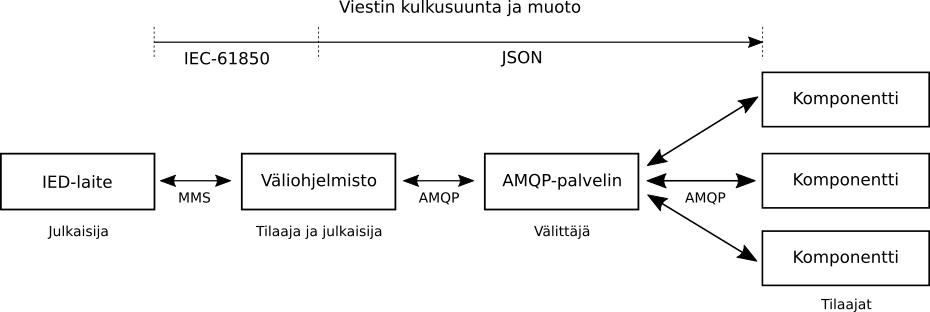
\includegraphics[width=1\textwidth]{pictures/high-level-system-architecture.png}
	\caption{Suunniteltu korkean tason järjestelmän hajautus ja kommunikointiprotokollat osapuolten välillä.}
	\label{fig:high-level-system-architecture}
\end{figure}

Arkkitehtuurissa väliohjelmisto tilaa viestejä IED-laitteelta IEC 61850 -standardin mukaisesti MMS-protokollan avulla. Viesti päädyttiin muuttamaan JSON-formaattiin helpomman luettavuuden saamiseksi ja sen muuntamisen hoitaa väliohjelmisto. Välittäjän kommunikointiprotokollaksi valittiin AMQP-standardi ja kommunikointiparadigmaksi jul\-kai\-si\-ja-ti\-laa\-ja ja viestijono. Väliohjelmisto tilaa viestejä IED-laitteelta ja uudelleenjulkaisee ne JSON-muodossa välittäjälle. Järjestelmän muut komponentit tilaavat viestejä välittäjältä AMQP-standardin mukaisesti. Suunniteltua mallia tullaan tarkentamaan teknisesti ennen toteutusta luvussa \ref{ch:suunnittelu}.
\chapter{Demoversion toiminta ja analyysi}
\label{ch:demo-analysis}
Ennen tämän työn aloitusta diplomityön tekijä oli kehittänyt ohjelmiston, joka kykeni viestien tilaukseen ja tallentamiseen. Ohjelma oli tarkoitettu demoksi tai prototyypiksi ennen varsinaista toteutusta. Demon tarkoituksena oli opettaa tekijälle IEC 61850 -standardia, todentaa viestien tilaamisen mahdollisuus ja tuoda esille toteutukseen liittyviä ongelmia. Ohjelma kykeni tilaamaan viestejä yhden IED-laitteen kaikilta RCB-instansseilta, prosessoimaan viestit ja tallentamaan ne relaatiotietokantaan.

Demoa ei ollut mahdollista käyttää tuotannossa osana muuta järjestelmää sen arkkitehtuurin ja toiminnan epävarmuuden takia. Tässä kappaleessa käydään läpi demon toimintaa ja siihen liittyviä ongelmia. Demosta on tarkoitus analysoida sen toiminnan epävarmuutta ja saada selville mistä se mahdollisesti johtui. Saatuja tietoja käytetään luvussa \ref{ch:suunnittelu} apuna uuden version suunnittelussa.


\section{Arkkitehtuuri}
\label{ch:demoversio-ja-sen-toiminta}
Demoversio oli ohjelmoitu Ruby-ohjelmointikielellä. Kuvassa \ref{fig:demo-architecture} on esitetty demoversion arkkitehtuuri korkealla tasolla ja kuinka viesti IED-laitteelta siirtyy tietokantaan. Yksi ajettu demoversion prosessi pystyi tilaamaan yhden IED-laitteen kaikki RCB-luok\-ki\-en instanssit. Instanssien tiedot luettiin relaatiotietokannasta. Ohjelmisto prosessoi viestit ja tallensi ne relaatiotietokantaan myöhempää käyttöä varten. Ruby-ohjelmistossa tärkeässä osassa oli \emph{libIEC61850}-kirjasto \cite{libIEC61850-homepage}. libIEC61850-kirjasto on avoimen lähdekoodin C-kielellä toteutettu kirjasto, joka abstrahoi IEC 61850 -standardin matalan tason määrittämiä palvelukutsuja ja datarakenteita helppokäyttöiseksi rajapinnaksi. Kirjasto tarjosi toiminnallisuuden IED-laitteella olevan palvelinohjelmiston sekä IED-laitetta käyttävän asiakasohjelmiston toteuttamiseen. IED-laitteen palvelimelle kirjasto tarjosi funktioita ja rakenteita standardin määrittämien luokkien hierarkian rakentamiseen ja käsittelyyn. IED-laitteen asiakasohjelmalle kirjasto tarjosi funktioita ja rakenteita standardin määrittämiin palveluihin, kuten arvojen lukuun ja asettamiseen, datajoukkojen käyttöön ja viestien tilaamiseen. Demoa toteutettiin käyttäen oikeaa IED-laitetta, joten kirjastosta tarvittiin vain sen asiakasohjelman ominaisuudet. Demon toteutuksen aikana kirjasto todettiin hyväksi vaihtoehdoksi ja sitä päätettiin käyttää myös uuden version toteutuksessa.

\begin{figure}[ht!]
	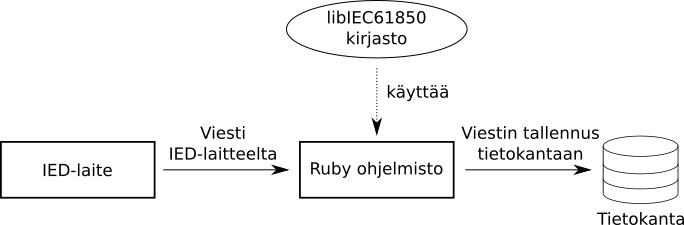
\includegraphics[width=0.8\textwidth]{pictures/demo-architecture.png}
	\caption{Ruby:lla toteutetun demoversion arkkitehtuuri ja tiedonsiirto.}
	\label{fig:demo-architecture}
\end{figure}

LibIEC61850-kirjasto on rakennettu käyttämään MMS-protokollaa tiedonsiirrossa IED-laitteen ja sen asiakasohjelman välillä IEC 61850 -standardin mukaan. Kuvassa \ref{fig:libiec61850-layer-architecture} on esitetty kirjaston kerrosarkkitehtuuri asiakasohjelmalle. Kirjastoon on toteutettu \emph{laiteabstraktiokerros} (\emph{Hardware Abstraction Layer}, \emph{HAL}). HAL:in avulla kirjasto voi toimia monella eri laitealustalla, ja käyttäjä voi tarvittaessa lisätä oman HAL-implementaation. Demoversiota suoritettiin Linux-käyttöjärjestelmällä, joten kirjastosta käytettiin olemassa olevaa Linux HAL -toteutusta. Kuvassa \ref{fig:libiec61850-layer-architecture} on punaisella merkitty laatikot, jotka kirjaston käyttäjä voi tarjota itse, keltaisella kirjaston uudelleenkäytettävät MMS-protokollan osuudet ja sinisellä IEC 61850 -standardin toteuttavat osuudet. Kuvaan on merkitty vihreällä demoon toteutetut osuudet, eli Ruby-kielelle liitos C-kieleen ja tämän päälle Ruby:lla toteutettu ohjelmisto.

\begin{figure}[ht!]
	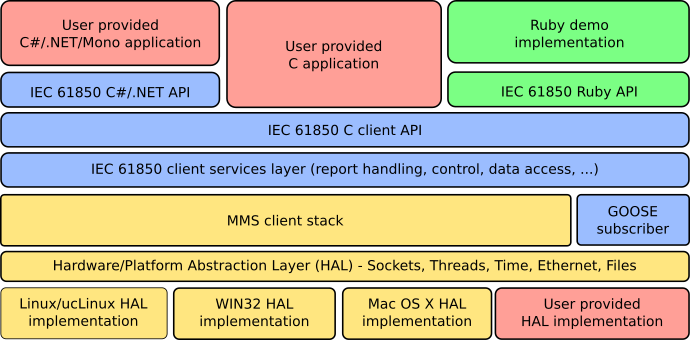
\includegraphics[width=1\textwidth]{pictures/libiec61850-layer-architecture.png}
	\caption{LibIEC61850-kirjaston kerrosarkkitehtuurin komponentit, vihreällä Ruby toteutukseen lisätyt osat (pohjautuu kuvaan \mbox{\cite{libIEC61850-api-overview}}).}
	\label{fig:libiec61850-layer-architecture}
\end{figure}

Ruby-koodista C-kielen funktioiden kutsuminen ei ole suoraan mahdollista, vaan kielten väliin täytyy toteuttaa liitos. Demoversiossa liitos oli tehty käyttäen Ruby:lle saatavaa \emph{ruby-ffi}-kirjastoa \cite{ruby-ffi-repo} (\emph{Foreign Function Interface}, \emph{FFI}). Liitoksen avulla Ruby voi kutsua C-kielen funktioita ja käyttää sen struktuureita ja muuttujia. Demossa kirjasto huolehti matalan tason IEC 61850 asiat, ja Ruby-osuus keskittyi liitoksen avulla viestien tilaamiseen, käsittelyyn ja tallentamiseen.


\section{Toiminta}
\label{ch:ongelmakohdat-ja-analysointi}
Ohjelman toiminta on esitetty sekvenssikaavioissa \ref{fig:sequence-diagram-report-subscription} ja \ref{fig:sequence-diagram-report-subscription-processing}. Sekvenssikaavio \ref{fig:sequence-diagram-report-subscription} jatkuu kuvassa \ref{fig:sequence-diagram-report-subscription-processing}. Kuvissa ohjelman kaksi eri silmukkaa on esitetty loop-laatikoilla. Sekvenssikaaviossa osallisena ovat tietokanta, Ruby-ohjelma, libIEC61850-kirjasto, libIEC61850-kirjaston natiivisäie ja IED-laitteen palvelinohjelma. Kirjaston natiivisäie on vastuussa yhteyden ylläpidosta ja datan siirtämisestä IED-laitteen ja kirjastoa käyttävän prosessin välillä. Sekvenssikaavioon on merkitty paksulla suorituksessa olevat palkit, esimerkiksi IED-laitteen palvelinohjelmisto on koko ajan suorituksessa. Tulevassa tekstissä ohjelman toiminta käydään pääpiirteittäin läpi ja kuvien numeroihin viitataan.

IED-laiteella viestejä mahdollisesti generoidaan ja lähetetään samaan aikaan. Seurauksena niitä voi saapua libIEC61850-kirjastolle ennen kuin edellinen viesti on käsitelty. Tätä varten kirjasto toteuttaa sisäisen puskurin viestien vastaanottamiseen. Puskurista prosessoidaan seuraava viesti, kun edellinen on prosessoitu. Toisin sanoen kirjasto ottaa viestejä vastaan sitä mukaa kun ne saapuvat ja ottaa niitä puskurista yksi kerrallaan saapumisjärjestyksessä. Kirjasto varaa yhden puskurin avattua yhteyttä kohti. Jos ohjelma avaa vain yhden yhteyden, kirjaston käyttäjän ei tarvitse huolehtia rinnakkaisuudesta. \cite{libIEC61850-repo}

\begin{figure}
	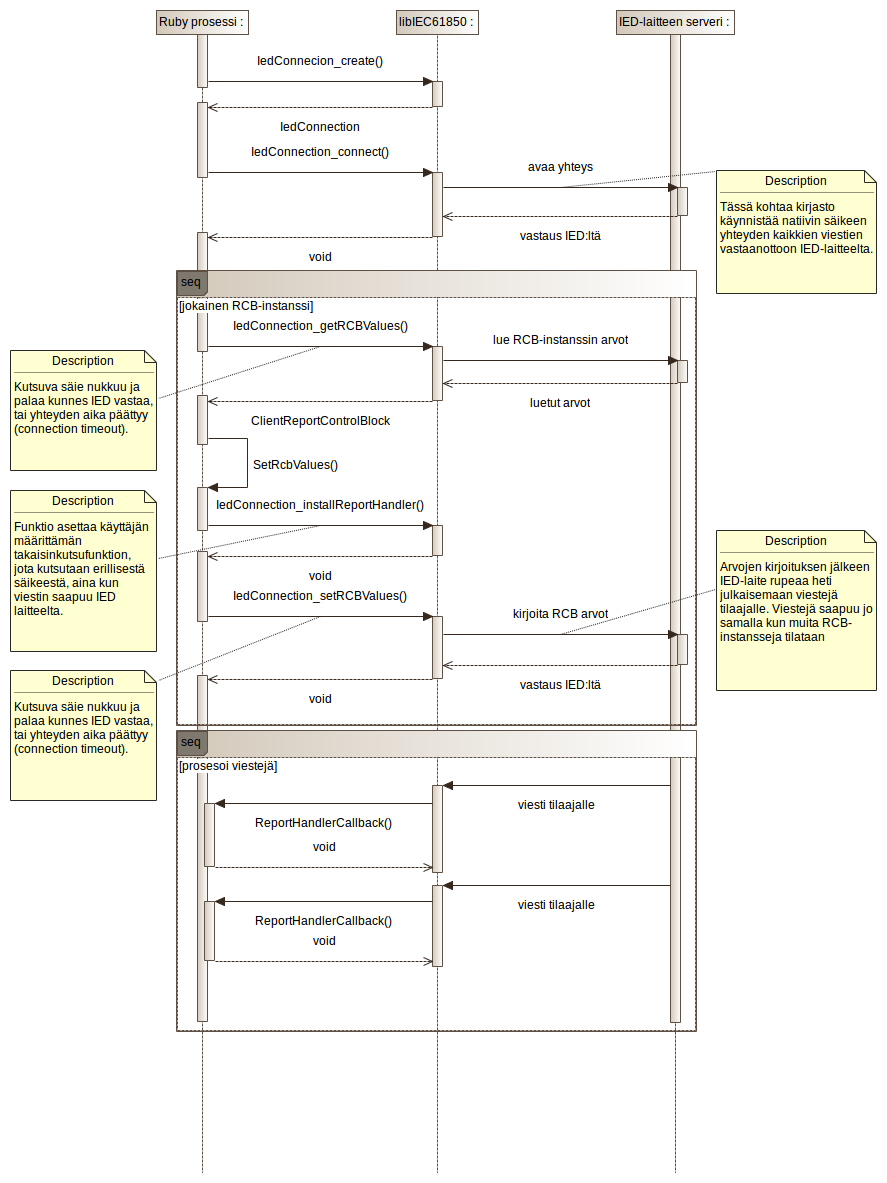
\includegraphics[width=1\textwidth]{pictures/sequence-diagram-report-subscription.png}
	\caption{Sekvenssikaavio kuinka Ruby-ohjelma avaa yhteydet ja tilaa kaikki IED-laitteen RCB-instanssit (jatkuu kuvassa \ref{fig:sequence-diagram-report-subscription-processing}).}
	\label{fig:sequence-diagram-report-subscription}
\end{figure}

\begin{figure}
	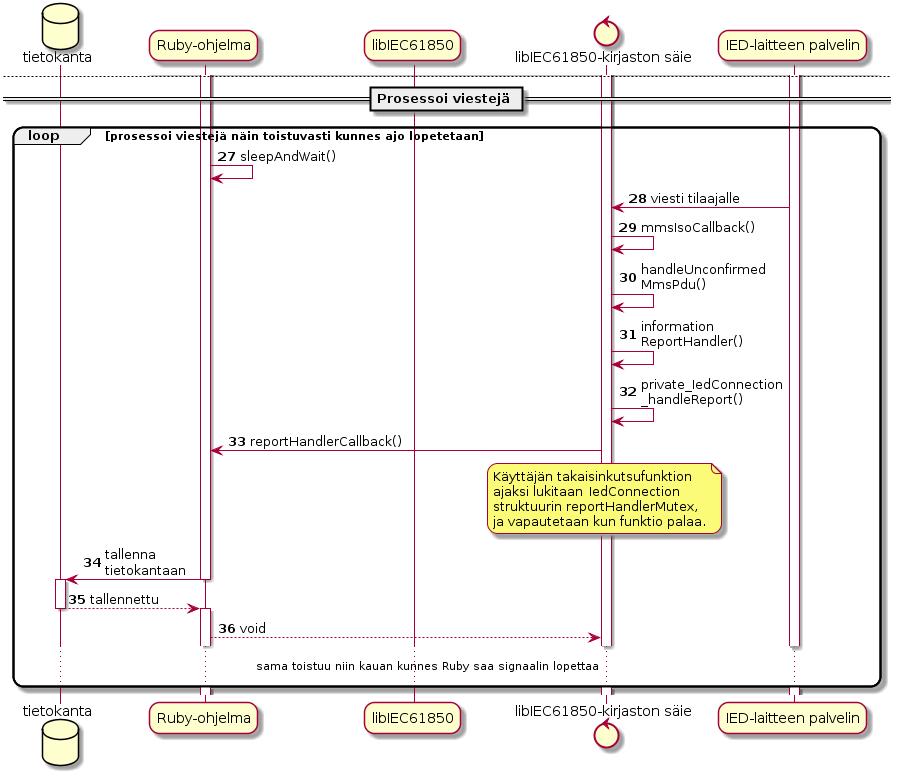
\includegraphics[width=1\textwidth]{pictures/sequence-diagram-report-subscription_001.png}
	\caption{Sekvenssikaavio kuinka Ruby-ohjelma prosessoi ja tallentaa viestejä libIEC61850-kirjastoa käyttäen (jatkoa kuvalle \ref{fig:sequence-diagram-report-subscription}).}
	\label{fig:sequence-diagram-report-subscription-processing}
\end{figure}

Ensimmäisenä ohjelma luki tietokannasta IED-laitteen, sekä sen kaikki RCB-instanssien tiedot. IED-laitteen tietojen avulla ohjelma muodosti yhteyden IED-laitteelle (kohdat 3--11). Tässä vaiheessa libIEC61850-kirjasto käynnistää erillisen natiivisäikeen yhteyden viestien vastaanottoon. Tätä säiettä kirjasto käyttää tulevien viestien vastaanottoon ja lähettämiseen. Yhteyden muodostuksen jälkeen ohjelma käy läpi silmukassa jokaisen IED-laitteen RCB-instanssin ja tilaa ne. RCB-instanssien tilaus tapahtuu kohdissa 12--26. Osa varausprosessia on instanssin arvojen luku ja takaisinkutsufunktion asettaminen, jota kirjasto kutsuu viestin saapuessa. \mbox{\cite{libIEC61850-repo}}

RCB-instanssin arvojen kirjoituksen jälkeen tilaus alkaa ja IED-laite aloittaa viestien lähettämisen (kohta 23). Seurauksena on, että ohjelma joutuu käsittelemään viestejä samalla kun muita RCB-instansseja varataan. Toisin sanoen asetettu takaisinkutsufunktio suoritetaan (kohdat 28--36). Kirjasto käytti samaa lukitusta takaisinkutsufunktion asettamisen ja sen suorituksen ajaksi. Nämä tapahtuvat kohdissa 19--20 ja 33--36. Tilauksen jälkeen ohjelma jää odottamaan viestejä vastaan ja asetettu takaisinkutsufunktio prosessoi viestit ja tallentaa ne tietokantaan. \mbox{\cite{libIEC61850-repo}}


\section{Ongelmien analyysi}
Demo oli toteutettu käyttäen \emph{Ruby on Rails} -kehystä, lyhennetään \emph{RoR}. RoR on tarkoitettu web-sovellusten kehittämiseen Ruby-kielellä. Demo toteutettiin suoritettavaksi RoR-kehyksen tarjoamalla erillisen Ruby-koodin suorituksen mekanismilla \cite{rails-runner}. Mekanismi sallii Ruby-koodin suorituksen RoR:in kontekstissa. Konteksti salli järjestelmän kirjastojen ja koodien käytön demossa. Huonona puolena tässä oli, että yksinkertaisen ohjelman suoritus vaatii järjestelmän kontekstin muistiin lataamisen ennen suoritusta. Tästä seurauksena yksi suoritettu demon prosessi varasi muistia noin 150 Mt, verrattuna uuteen RoR-projektiin, joka vei noin 67 Mt muistia. Ohjelman yksinkertaisuuteen nähden varatun muisti määrä on suuri ja sitä olisi mahdollista pienentää.

Demossa isoimpana ongelmana oli sen huono suorituskyky ja toiminnan epävarmuus RCB-instanssien määrän ollessa esimerkiksi noin 10. RCB-instanssien määrän ollessa liian suuri ohjelma saattoi epäonnistua osan tilaamisessa, koska yhteys aikakatkaistiin arvojen kirjoituksessa. Lisäksi ongelmaksi muodostui usean RCB instanssin tilaamisen kulunut aika. Yhteensä aikaa saattoi kulua noin 30 sekuntia 10 instanssin tilaamiseen. RCB-instanssien määrä vaihtelee IED-laitteen mukaan. Tässä työssä käsitellyt määrät olivat 3--13 instanssia.

Huonoon suorituskykyyn oli pääasiassa syynä Ruby-oletustulkissa (versiosta 1.9 eteenpäin \emph{Yet another Ruby VM}, \emph{YARV}) oleva \emph{globaali tulkkilukitus} (\emph{Global Interpreter Lock}, \emph{GIL}, tai \emph{Global Virtual Machine Lock}, \emph{GVL}). GIL pakottaa Ruby-ohjelman ajoon vain yhdellä ytimellä ja vain yksi säie vuorossa kerrallaan ja on täysin riippumaton käyttöjärjestelmän vuorottajasta \mbox{\cite[s.~131--133]{Odaira2014}}. Seurauksena tästä on, että tilanteessa jossa Ruby-koodi on tilaamassa RCB-intanssia ja samalla hetkellä IED-laite lähettää viestin. LibIEC61850-kirjasto kutsuu Ruby:n puolella olevaa takaisinkutsufunktiota ja sen suorituksen ajaksi GIL lukitaan. Toisin sanoen RCB-instanssia tilaava Ruby-koodin suoritus pysähtyy takaisinkutsufunktion ajaksi. Seurauksena on loppujen RCB-instanssien hidas tilaaminen ja yhteyden aikakatkaisut, jos vaihto tapahtuu oikeaan aikaan.

Kuvassa \ref{fig:ruby-gil} on esitetty kuinka Ruby-tulkki vuorottaa kahta ajossa olevaa säiettä. Kuvassa demon Ruby-koodi kutsuu \texttt{Ied""Connection""\_set""RCB""Values()} funktiota, ajo jää kesken ja tapahtuu vaihto, koska viesti saapui. Takaisinkutsufunktio suoritetaan ja suoritus palaa takaisin aikaisempaan funktion suoritukseen. Tässä vaiheessa, jos vaihto on huonolla hetkellä ja kesti liian kauan, tulee yhteyden aikakatkaisu ja RCB-instanssi jää tilaamatta.

Huonoon suorituskykyyn mahdollisesti vaikutti myös lukitus \texttt{report""Handler""Mutex}, jota kirjastossa käytetään, kun takaisinkutsufunktio asetetaan tai sitä suoritetaan. Lukitus aiheuttaa säikeen nukkumisen niin kauan kunnes lukitus vapautuu. Tässä tapauksessa, jos viestin prosessointi kestää liian kauan (kuvassa \ref{fig:sequence-diagram-report-subscription-processing} kohdat 33--36) ja samalla tilataan muita RCB-instansseja (kuvassa \ref{fig:sequence-diagram-report-subscription} kohdat 12--26). Säie joutuu odottamaan lukituksen vapautusta takaisinkutsufunktion asettamisen ajan (kohdat 19--20). Ratkaisuna tähän olisi pitää takaisinkutsufunktio mahdollisimman lyhyenä suoritusajan suhteen. Ruby-kieli on tulkattava kieli verrattuna libIEC61850-kirjaston käännettyyn C-kieleen. Tulkattavan kielen suorituskyky on huonompi kuin valmiiksi konekäskyiksi käännetyn kielen. Edellä mainittujen lisäksi tämä saattoi myös vaikuttaa ohjelman suoritukseen. \mbox{\cite{Kozlovski2017, Storimer2013}}

\begin{figure}[ht!]
	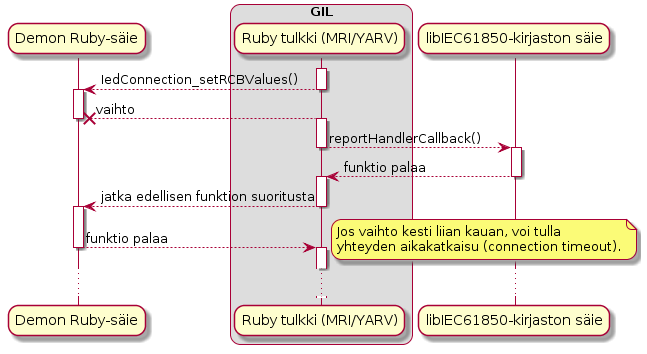
\includegraphics[width=1\textwidth]{pictures/ruby-gil.png}
	\caption{Ruby-tulkin globaalin lukituksen toiminta, joka vuorottaa ajossa olevia säikeitä riippumatta käyttöjärjestelmän vuorottajasta.}
	\label{fig:ruby-gil}
\end{figure}

Demototeutuksessa oli muistivuoto huonon ohjelmoinnin tuloksena. Muistivuoto on tilanne missä ohjelma varaa lisää muistia ilman, että sitä vapautetaan takaisin käyttöjärjestelmälle. Muistivuoto johtui todennäköisesti ohjelmointivirheestä ruby-ffi -kirjastolla. Kun liitos Rubysta tehdään C-kieleen, täytyy ohjelmoijan miettiä varatun muistin vapauttamista. Ruby-ohjelmoijan ei normaalisti tarvitse tästä huolehtia automaattisen roskien keruun ansiosta. Muistivuoto havaittiin kun ohjelma jätettiin suoritukseen pitemmäksi aikaa ja se oli varannut melkein kaiken käyttöjärjestelmän muistista itselleen. Tämän pystyi havaitsemaan helposti ohjelman suorituksen aikana Linuxin htop-ohjelmalla MEM\%-sarakkeesta. Sarake kertoo prosessin käyttämän prosentuaalisen osuuden koko käyttöjärjestelmän muistista \cite{htop-user-guide}. Luku kasvoi tasaisesti ja sen verran nopeasti, että sen havaitseminen oli mahdollista ilman pitempää suoritusaikaa.


\section{Yhteenveto}
Demon jatkokehitys toimivaksi olisi vaatinut paljon vaivaa huomioon ottaen edellä käsitellyt ongelmat. Tämän lisäksi sen kehityksessä ei ollut huomioitu järjestelmän hajautuksen vaatimuksia. Tiedon jakaminen muun järjestelmän kanssa tietokannan kautta ei ole hyvä ratkaisu. Se johtaisi tilanteeseen missä järjestelmän komponentit lukisivat viestejä tietokannasta jatkuvasti, ilman tietoa milloin uusi viesti on saapunut. Tästä aiheutuu turhaa kuormaa tietokannalle ja komponentin saama tieto ei välttämättä ole ajan tasalla. Isoilla muutoksilla demo olisi ollut mahdollista saada täyttämään asetetut vaatimukset ja sen ongelmat korjattua. Demo kuitenkin päätettiin korvata kokonaan uudella toteutuksella sen vaatiman työmäärän takia.

Ohjelmiston huonoon suorituskykyyn ja epävarmuuteen pääasiassa on syynä Ruby-kielen GIL. Varatun muistin määrän oli suuri yksinkertaista ohjelman ajamista varten. Syynä todennäköisesti oli RoR-kehyksen ajoympäristö, joka latasi muistiin muuta järjestelmää ja sen kirjastoja. Ohjelmassa oli muistivuoto, joka todennäköisesti johtui Ruby:n ja C-kielen liitoksen huonosta ohjelmoinnista. Tässä luvussa saatuja tietoja tullaan käyttämään suunnitelussa luvussa \ref{ch:suunnittelu}. Demototeutuksen perusteella libIEC61850-kirjasto todettiin hyväksi ja sitä käytettiin myös uudessa versiossa. Suunnittelussa kysymyksenä jää miettiä mitkä tekniikat valitaan toteutukseen, jotta suorituskykyongelmat vältetään ja varatun muistin koko pidetään kohtuullisena. Muistivuoto ohjelmassa taas vältetään huolellisella ohjelmoinnilla.
\chapter{Suunnittelu}
\label{ch:suunnittelu}
\begin{it}
	Pitäisikö tähän kirjoittaa ohjelman ajosta ja siihen liittää sekvenssikaavio perustoimminnasta? Kirjoita jos tuntuu että tarvetta.
\end{it}
Tässä osuudessa käydään toteutetun ohjelman suunnittelu läpi ja kerrotaan miten ja miksi ratkaisuihin päädyttiin. Kappaleissa vertaillaan eri vaihtoehtoja ja peilataan demoversion ongelmia ja niiden perusteella yritetään löytää toimiva ratkaisu ongelmaan. Ensin suunnitellusta ohjelmasta annetaan kattava kokonaiskuva lukijalle ja tämän jälkeen tulevissa kappaleissa mennään jokaisen kohdan yksityiskohtiin tarkemmin.


\section{Kokonaiskuva}
Aikaisemmin kappaleessa \ref{ch:demoversio-ja-sen-toiminta} kuvassa \ref{fig:demo-architecture} esiteltiin demoversion arkkitehtuuri ja sen toiminta. Kuinka viestit IED-laitteelta kulkee ohjelman läpi ja tallennetaan tietokantaan. Tietokannasta muut ohjelmat lukevat tietoa kyselemällä sitä erikseen. Suunnittelun jälkeen demoversion järjestelmästä päätyttiin kuvassa \ref{fig:planned-system-architecture} olevaan järjestelmän arkkitehtuuriin. Kuvassa katkoviivalla on merkitty tässä kappaleessa suunniteltu ohjelmisto. Ja kuvan yläreunassa oleva viiva kuvaa viestin kulkua järjestelmän eri osapuolten läpi ja missä muodossa viesti on missäkin kohtaa.

\begin{figure}[ht!]
	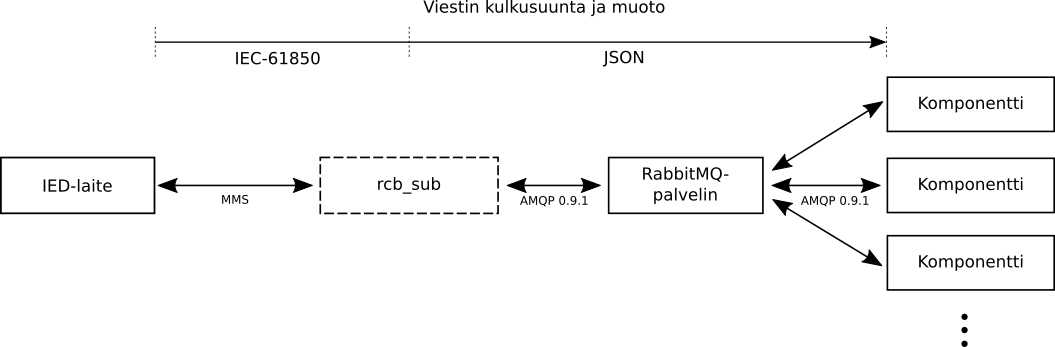
\includegraphics[width=1\textwidth]{pictures/planned-system-architecture.png}
	\caption{Suunnitellun järjestelmän toiminta ja viestin kulkeminen ja muoto eri osapuolten välillä.}
	\label{fig:planned-system-architecture}
\end{figure}

Suunnitellussa arkkitehtuurissa C-kielellä toteutettu ohjelma on komentorivipohjainen ja ei käyttänyt tietokantaa. Kaikki ohjelman ajoon annettavat parametrit annetaan komentoriviparametreille ennen ohjelman käynnistämistä, verrattuna demoversion toteutukseen, joka luki tiedot tietokannasta. C-ohjelma voi tilata yhdellä IED-laitteella olevia RCB-instansseja. Tilattuaan RCB-instanssit, ohjelma odottaa viestejä IED-laitteelta IEC 61850 -standardin määrittämässä muodossa. Kun viesti saapuu, ohjelma prosessoi sen ja julkaisee AMPQ-standardin pohjaiselle jonopalvelimelle JSON-muodossa (engl. JavaScrip Object Notation). Lopullisessa toteutuksessa jonopalvelimena käytettiin RabbitMQ-nimistä ohjelmistoa, joka pohjautuu AMPQ-standrdin versioon 0.9.1. Jonopalvelimelta muut tilaavat ohjelmat voivat tilata viestejä, ja viestin saapuessa palvelin ilmoittaa siitä asiakkaalle. Toteutettu C-ohjelmisto käytti edelleen demoversiosta tuttua libiec61850-kirjastoa hoitamaan matalan tason IEC 61850 -standardin määrittämän funktionaalisuuden.


\section{Järjestelmän hajautus ja arkkitehtuuri}
\label{ch:järjestelmän-hajautus-ja-arkkitehtuuri}
Järjestelmän hajauttaminen oli vaatimus uudelle arkkitehtuurille, joka täytyisi ottaa huomioon. Hajautuksella tarkoitetaan että viesteistä kiinnostuneet ohjelmat, pystyisivät niitä tilaamaan ja ottamaan vastaan helposti. Ongelmia ei saisi tulla jos asiakasohjelmia olisi tulevaisuudessa enemmänkin. Demossa erilliset ohjelmat joutuivat lukemaan viestejä jatkuvasti tietokannasta, ilman tietoa siitä milloin uusi viesti olisi saapunut. Tällainen ratkaisu ei tulisi toimimaan pitemmän päälle ja tilanne olisi pahentunut jos tietoa tarvitsevia ohjelmia olisi enemmänkin tulevaisuudessa. Lisäksi tässä toteutuksessa tietokanta on jatkuvan turhan lukemisen ja kuormituksen kohteena. Tilanteeseen tarvittaisiin ratkaisu, jossa tilaava ohjelma voisi tilata viestin ja saada ilmoituksen kun tieto on saatavilla, tilaaja-julkaisija -arkkitehtuuri.

Ratkaisuna olisi voinut ajatella että tietoa tarvitsevat ohjelmat, olisi voineet suoraan tilata viestit IED-laitteelta. Näin kaikki ohjelmat saisivat saman viestin. Kuitenkin tässä esteenä on, että IEC 61850 -standardin määrityksen mukaan yksi RCB-instanssi voi olla vain tilattuna yhdellä asiakkaalle kerrallaan, niinkuin teorian kappaleessa \ref{ch:viestien-tilaus-ja-tilauksen-konfigurointi} käsiteltiin. Ja IED-laitteiden RCB-instanssit ovat rajalliset ja päätetty laitteen konfiguroinnin yhteydessä. Lisäksi IED-laitteet pystyvät rajoittamaan päällä olevien yhteyksien määrää johonkin lukuun. Tavoitteena siis olisi minimoida avoimet yhteydet IED-laitteelle, ja samalla tarjota sama viesti mahdollisimman monelle siitä kiinnostuneelle ohjelmalle. Näistä vaatimuksista päästään ratkaisuun, missä yksi ohjelma tilaa kaikki halutut RCB-instanssit yhdeltä IED-laitteelta. Odottaa viestejä ja lähettää ne edelleen muille niitä tarvitseville ohjelmille. Viestejä tarvitsevien ohjelmien määrä voi vaihdella tarpeen mukaan. Tästä päästään vaatimukseen, että IED-laitteelta viestejä tilaavan ohjelmiston ei tarvitsisi tietää muista tilaavista ohjelmista mitään. Ohjelman pitäisi pystyisi julkaisemaan viestit eteenpäin, välittämättä siitä kuka viestejä vastaanottaa.

Ratkaisuna yllä mainittuihin vaatimuksiin oli sijoittaa IED-laitteen ja muiden tilaavien ohjelmien väliin väliohjelmisto, kuten kuvassa \ref{fig:planned-system-architecture} on C-ohjelma sijoitettu. Näin pystyttiin minimoimaan yhteyksien määrä IED-laitteelle yhteen. Lisäksi sijoittamalla C-ohjelman ja muiden tilaavien ohjelmien väliin jonopalvelin, saadaan aikaan joustavuus mitä haluttiin. C-ohjelman ei tarvitse välittää siitä kuka viestejä vastaanottaa ja jonopalvelimen avulla yhden julkaisijan voi tilata monta erillistä tilaaja. Jonopalvelimen avulla jokainen tilaaja saa saman alkuperäisen viestin, mutta kopiona. Koska standardi ei määrittänyt muita viestien tilaamisen mahdollisuuksia, tämä suunnitelma arkkitehtuurista täytti kaikki sille asetetut vaatimukset.

Demoversiossa ohjelma luki IED-laitteen tiedot kuten IP-osoitteen ja RCB-instanssien referenssit tietokannasta ja tallensi saapuneet viestit tietokantaan. Nyt kun viestit julkaistiin erilliselle jonopalvelimelle, niin tietokantaa ei siihen enää tarvinnut. C-ohjelman tarkoitus oli vain olla väliohjelma viestien välittämiseen eteenpäin, joten siihen ei tarvittu käyttöliittmääkään. Ohjelmasta päätettiin tehdä komentorivipohjainen toteutus, jolle kaikki tiedot voitaisiin syöttää komentorivillä parametereillä käynnistyksen yhteydessä. Tällä suunnitelmalla toteutus ei tarvitsisi tietokantaa ollenkaan, joten se voitiin tiputtaa pois suunnitelmasta.


\section{Suorituskyky ja kielen valinta}
Demoversio oli ohjelmoitu Ruby-kielellä ja siinä oli paikoin suoritukseen liittyviä ongelmia ja epävarmuutta, etenkin viestien ja RCB-instassien määrän olessa suurempi. Syitä ja ongelmia käytiin läpi kappaleessa \ref{ch:ongelmakohdat-ja-analysointi}. Oli selvää että ohjelman suorituskykyä täytyi saada parannettua ja siinä olevat ongelmat korjattua esimerkiksi muistivuoto. Ennen koko ohjelman uudelleenkirjoitusta, Ruby-ohjelmaa kokeiltiin saada toimimaan JRuby\footnote{\url{http://jruby.org/}} nimisellä Ruby-tulkilla. Tavoitteena saada demoversion toteutus toimimaan ilman GIL:iä ja säikeet suoritukseen rinnakkain. JRuby on Ruby-koodin tulkki, joka suorittaa Ruby-lähdekoodia Java virtuaalikoneen (engl. Java Virtual Machine, lyhennetään JVM) päällä. JRuby mahdollistaa säikeiden suorituksen rinnakkain JVM:n omilla säikeillä ja näin ollen suorituksen pitäisi olla nopeampaa \cite{Youssef2013}. Jos tämä lähtökohta olisi toiminut, olisi edelleen järjestelmän arkkitehtuuria pitänyt muuttaa samaan suuntaan, kuin kappaleessa \ref{ch:järjestelmän-hajautus-ja-arkkitehtuuri} kuvattiin. Tämän lisäksi demossa oleva muistivuoto olisi pitänyt korjata. JRuby ei kuitenkaan toiminut ja nopean yrityksen jälkeen päätettiin vain palata suunnitelmaan kirjoittaa koko ohjelma uudestaan. Syynä tähän oli että demoversio oltiin tehty osaksi isompaa Rails projektia, joka toimi Rubyn oletustulkin päällä. Ja JRuby ei tukenut kaikkia projektin kirjastoja mitä se käytti. Rubyssä kirjastoja kutsutaan jalokiviksi (engl. gem). Seurauksena olisi ollut saman projektin ylläpitäminen kahdelle eri tulkille tai asennettavien pakettien erottaminen. Kuitenkaan yrittämisen jälkeen tätäkään ei saatu toimimaan loppupelissä. Kysymksenä tämän aikana tuli ajan käyttö ja fakta että demosta olisi pitänyt korjata ja paikata monta asiaa. Päätyttiin toteuttamaan koko ohjelmisto uudestaan erillisellä kielellä jossa ei olisi suorituskykyongelmia. Samalla uudessa toteutuksessa ohjelman pystyi alusta asti tekemään asetetut tavoitteet mielessä ja demoversion ongelmia ei tarvitsisi korjata.

Uuden toteutuksen kieleksi valittiin C-kieli. Isona syynä kielen valintaan oli tekijän iso mieltymys matalan tason ohjelmointiin ja C-kieleen. Lisäksi C-kieli käännetään alustalle suoraan konekäskyiksi, joiden suoritus on nopeampaa kuin tulkattavan kielen, kuten Ruby ja Python. Kielen valinnan yhteydessä kuitenkin oli hyvä varmistaa kaikkien suunniteltujen liitosten mahdollisuus. C-kielelle löytyi kirjastoja RabbitMQ-jonopalvelimen käyttämiseen ja lisäksi JSON rakenteen muodostamiseen. Hyötynä vielä C-kielen valinnasta oli, että demossa käytettyä libIEC61840 kirjastoa pystyi käyttämään suoraan ilman erillistä liitosta, koska kirjasto oli myös tehty C-kielellä. Tarkemmin käytettyihin kirjastoihin ja toteutukseen mennään kappaleessa \ref{ch:toteutus}.


\section{Prosessoidun viestin muoto ja rakenne}
Saapuva viesti esitettiin libIEC61850-kirjastossa ClientReport struktuurin instanssina. Stuktuuri sisältää viestin datan ja sen voi lukea käyttämällä kirjaston tarjoamia funktioita \cite{libIEC61850-doc}. Saapunut viesti haluttiin jakaa jonopalvelimen läpi muille osapuolille, joten viestin täytyi olla helposti luettavassa muodossa muille ohjelmille. Viesti päädyttiin muuttamaan helposti ymmärrettäväksi JSON-rakenteeksi. JSON-rakenteen voi helposti ihminen lukea ja se on nykypäivänä paljon käytetty tiedonsiirtomuoto erilaisissa web-palveluissa ja rajapinnoissa. Myöskin JSON-rakenteiden lukemiseen on monelle eri kielellä olemassa valmiita kirjastoja sen monikäyttöisyyden takia \cite{Patrizio2016}.

Liitteessä \ref{ch:report-json-format} on esitetty prosessoidun JSON-rakenteen muoto johon tässä työssä päädyttiin. Ja minkä tässä työssä toteutettu C-ohjelma lopulta julkaisi RabbitMQ-jonopalvelimelle. Standardin määrittämää viestin rakennetta ja sisältöä käytiin läpi kappaleessa \ref{ch:viestin-rakenne}. JSONin rakenne pääasissa noudattaa standardin määrittämää viestin rakennetta, mutta joitakin asioita on tehty toisin. Lisäksi C-ohjelma myös lisäsi viestiin lisää tietoa attribuuteista selkeyden takia kuten viitteen, tyypin ja koon. Kuinka tämä toteutettiin käsitellään tarkemmin kappaleessa \ref{ch:toteutus}.

Standardin viestin kenttien määrää pystyi säätämään RCB-instanssin OptFlds-attribuutilla. JSONiin kuitenki haluttiin lisätä kaikki mahdolliset kentät selkeyden vuoksi. Joten jos kenttä viestistä puuttui, asetettiin sen arvoksi JSONissa null. Esimerkiksi liitteessä \ref{ch:report-json-format} kentän confRevision arvo on null. Eli tällöin RCB-instanssissa OptFlds-attribuutin conf-revision on olut epätosi. Sama käytäntö toistettiin kaikille muillekin vaihtoehtoisille kentille. Tällä periaatteella viestin OptFlds-kenttä voitiin jättää pois JSONista. JSON:iin päädyttin lisäämään FCD- ja FCDA-viitteiden alla viitatut oikeat attribuutien viitteet, tyyppit ja koot arvojen lisäksi. Tämä toteutettiin selkeyden takia, mitkä arvot oikeasti kuuluvat viestiin ja mitkä ovat niiden viitteet. Standardissa viesti sisälsi vain datajoukon FCD- tai FCDA-viitteen ja taulukon arvoja mitä sen alla viitattiin. Liitteessä \ref{ch:report-json-format} oleva JSONin rakenteessa ensimmäinen values-attribuutti on siis lista datajoukon FCD- tai FCDA-viitteitä ja siihen liittyvät kentät mitä viestin rakenteessa oli (kuva \ref{fig:iec61850-report-format}). Eli viestin Reason Code on laitettu reasonForInclusion attribuuttiin. Viestin DataRef-kenttä on pilkottu kolmeen eri kenttään mmsReference, reference ja functionalConstraint. Viestien viitteet tulevat MMS-protokollamäärityksen muodossa, eli pisteet (.) on korvattu dollarilla (\$) ja viite sisältää funktionaalisen rajoitteen. Nyt mmsReference sisältää viestin alkuperäisen MMS-viitteen, reference sisältää standardin abstraktin viitteen ja functionalConstraint sisältää funktionaalisen rajoitteen. Nämä on erotettu selkeyden takia, koska todennöisesti jotkin asiakasohjelmat tarvitsivat standardin käyttämää abstraktia viitettä. Tällä asiakasohjelma välttää teksimuunnokset. JSONin sisempi values-attribuutti sisältää taulukon itse viestin arvoista, mutta C-ohjelma lisäsi niihin niiden oikeat viitteet, tyypin ja koon. Poikkeuksena boolean ja utc-time tyypit, jolla ei ole kokoa ollenkaan. Koko kertoo monellako bitillä kyseinen attribuutti esitetään ja se voi vaihdella saman tyypin välillä (esimerkiksi bit-string). Myöskin bit-string tyypille päädyttiin lisäämään kaksi eri arvoa valueLittleEndian ja valueBigEndian. Tämä sen takia, koska tavujärjestys ei ole vältämättä tiedossa missä järjestyksessä bitit muuttujassa ovat. Päätettiin tarjota kummatkin vaihtoehdot asiakkaalle. Ajat päätettiin antaa suoraan siinä formaatissa ja tyyppinä mitä ne tulevat viestistä. Eli viestin päätason aikaleima on millisekunteja UNIX-ajanlaskun alusta 1. tammikuuta 1970 klo 00:00:00 UTC tähän hetkeen. Attribuuteissa tyypiltään utc-time, luku on sekunteja samasta UNIX-ajanlakusta tähän hetkeen \cite[s.~26--27]{IEC61850-7-2}.
\chapter{Toteutus}
\label{ch:toteutus}
Tässä osiossa käydään läpi kappaleessa \ref{ch:suunnittelu} suunniteltun ohjelman toteuttaminen. Toteutus alkaa yleiskuvalla sen komponenteista ja niiden toiminnasta. Yleiskuvan jälkeen mennään tarkemmin ohjelman yksityiskohtiin kuten kirjastoihin ja niiden toimintaan. Lopuksi mietitään jatkokehitysideoita, eli mitä olisi voinut lisätä, tehdä toisin ja mahdollisia puutteita.


\section{Yleiskuva}
\label{ch:rcb-sub-yleiskuva}
Työssä toteutetiin komentorivipohjainen ohjelma C-kielellä. Ohjelman tarkoitus oli tilata IED-laitteen viestit ja prosessoida ne JSON-muotoon RabbitMQ-palvelimelle. RabbitMQ:lta muut ohjelmat pystyivät tilaamaan JSON-viestejä. Kuvassa \ref{fig:rcb-sub-komponenttikaavio} on esitetty komponenttikaavio  toteutetusta ohjelmasta ja siihen käytetyistä kirjastoista. Toteutettu komponentti on kuvassa keskellä keltaisella ja nimeltään \emph{rcb\_sub}. Kuvasta voi nähdä miten eri komponentit ovat relaatiossa keskenään rcb\_sub-ohjelman kanssa. Kuvassa on myös esitetty IED-laite ja RabbitMQ-palvelin.

\begin{figure}[ht!]
	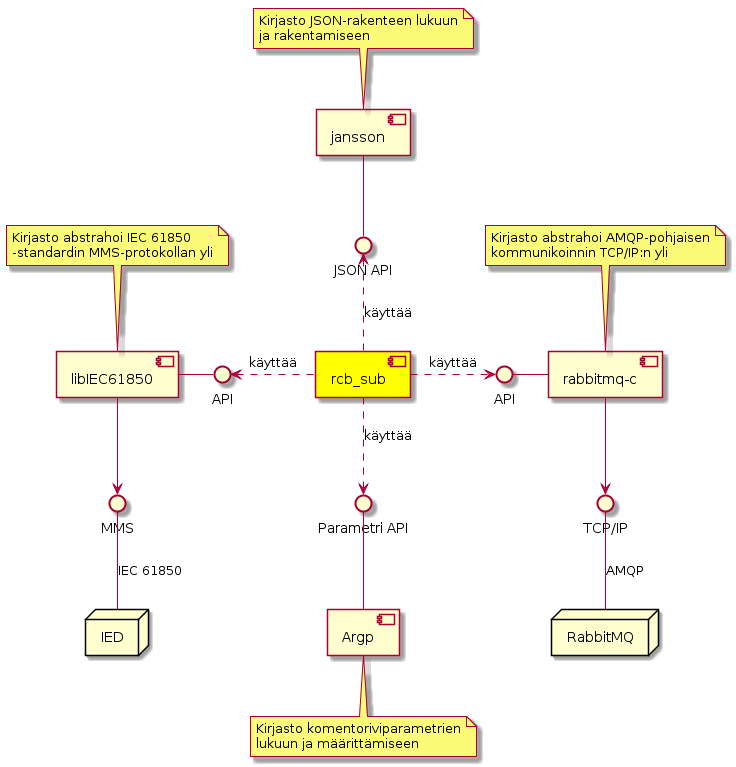
\includegraphics[width=1\textwidth]{pictures/rcb-sub-component-diagram.png}
	\caption{Toteutuksen komponenttikaavio sen osista ja relaatioista toisiinsa.}
	\label{fig:rcb-sub-komponenttikaavio}
\end{figure}

Toteutuksessa käytettiin seuraavia kirjastoja:
\begin{itemize}
	\item \emph{libiec61850},
	\item \emph{rabbitmq-c},
	\item \emph{jansson}, ja
	\item \emph{Argp}.
\end{itemize}
Kaikki käytetyt kirjastot on toteutettu C-kielellä, kuten rcb\_sub. Kirjastojen tarkoitus on abstrahoida jonkin asian käyttö, ja tarjota käyttäjälle siitä helppokäyttöinen ja ymmärrettävä rajapinta. Rajapintaa käyttämällä kirjasto hoitaa matalan tason toiminnan ilman, että sen käyttäjän tarvitsee siitä välittää. Libiec61850-kirjasto abstrahoi IEC 61850 -standardin käyttöä ja hoitaa matalan tason MMS-protokollan kommunikoinnin \mbox{\cite{libIEC61850-repo}}. Samaa kirjastoa käytettiin demoversiossa (kappale \ref{ch:demoversio-ja-sen-toiminta}) ja kirjaston kerrosarkkitehtuuri esitettiin aikaisemmin kuvassa \ref{fig:libiec61850-layer-architecture}. Kuvassa \ref{fig:rcb-sub-komponenttikaavio} libiec61850 kommunikoi suoraan IED-laitteen kanssa MMS-protokollaa käyttäen. Rabbitmq-c-kirjasto abstrahoi RabbitMQ-palvelimen käyttöä ja hoitaa matalan tason AMQP-pohjaisen kommunikoinnin \mbox{\cite{rabbitmq-c-repo}}. Toteutuksessa rabbitmq-c kommunikoi suoraan RabbitMQ-palvelimen kanssa. Jansson-kirjasto abstrahoi JSON-rakenteiden lukua ja käsittelyä C-kielelle \mbox{\cite{jansson-repo}}. Kirjastoa käytettiin rakentamaan IED-\-lait\-teel\-ta saapuneesta viestistä JSON-muotoinen viesti. JSON-rakenne on nähtävissä liitteessä \ref{ch:report-json-format}. Argp-kirjasto auttaa ohjelman komentoriviparametrien määrittämisessä ja käsittelyssä \mbox{\cite{argp-glibc-guide}}. Kirjasto auttaa toteuttamaan ohjelmalle \emph{UNIX}-tyyliset parametrit. Eli vaaditut parametrit ja vaihtoehtoiset lyhyet ja pitkä parametrit. Vaadituista parametreista esimerkiksi Linux:in komento \texttt{mv foo.txt bar.txt}, jossa \emph{foo.txt} ja \emph{bar.txt} ovat vaadittuja parametreja. Vaihtoehtoisista parametreista esimerkkinä pitkä muoto \texttt{-{}-bytes} ja lyhyt muoto \texttt{-b}. Lisäksi kirjasto lisää ohjelmaan automaattisesti Linux:ista käyttäjille tutut \texttt{-{}-help} ja \texttt{-{}-version} vaihtoehtoiset parametrit. Komennolla \texttt{-{}-help} kirjasto tulostaa Linux:ilta tutun ohjelman aputekstin käyttäjälle, jossa on esitetty ohjelman kaikki parametrit ja niiden selitteet \mbox{\cite{step-by-step-into-argp}}.

Kuvassa \ref{fig:rcb-sub-sekvenssikaavio} on esitetty rcb\_sub-ohjelman sekvenssikaavio pääpiirteisestä toiminnasta. Toteutus noudattaa suurinpiirtein samoja periaatteita kuin demo (kuva \ref{fig:sequence-diagram-report-subscription}). Tässä kohtaa käydään läpi ohjelman pääpiirteinen toiminta ja myöhemmin tarkemmin läpi kappaleessa \ref{rcb-sub-toiminta}. Ensin ohjelman suoritus alkaa lukemalla annetut parametrit Argp-kirjastolla (kohdat 1--2). Parametreissa tulee tiedot yhteyden muodostamiseen IED-laitteelle ja RabbitMQ-palvelimelle (kohdat 3--6). Parametreissa on myös tiedot RCB-instansseista jotka halutaan IED:ltä tilata. Yhteyksien muodostamisen jälkeen jokainen parametrina annettu RCB käydään läpi silmukassa ja sen arvot ja datajoukon viitteet luetaan IED:ltä (kohdat 7--12). Tämän jälkeen sisäkkäisessä silmukassa luetaan datajoukon viitteiden muuttujien \emph{spesifikaatiot} (kohdat 11--12). Spesifikaatio antaa tiedot muuttujien pituudesta ja tyypistä. Näitä tietoja käytettiin JSON-rakenteessa täydentämään viestiä (esimerkkinä liiteessä \ref{ch:report-json-format} rivit 21--22). Tämän jälkeen tehdään toinen silmukka, jossa jokainen RCB-instanssi tilataan ja niille asetetaan takaisinkutsufunktio (kohdat 13--16). Arvojen kirjoitushetkellä (kohta 15) RCB varataan ja se aloittaa viestien lähettämisen rcb\_sub-ohjelmalle. Jokaisen RCB:n kirjoituksen jälkeen ohjelma jää loputtomaan silmukkaan ottamaan viestejä vastaan (kohdat 17--22). Viestin saapuessa kutsutaan asetettua takaisinkutsufunktiota, jonka parametrina on saapunut viesti (kohta 17). Viesti muutetaan JSON-muotoon jansson-kirjastolla ja julkaistaan RabbitMQ-palvelimelle rabbitmq-c-kirjastolla (kohdat 18--21).

\begin{figure}[ht!]
	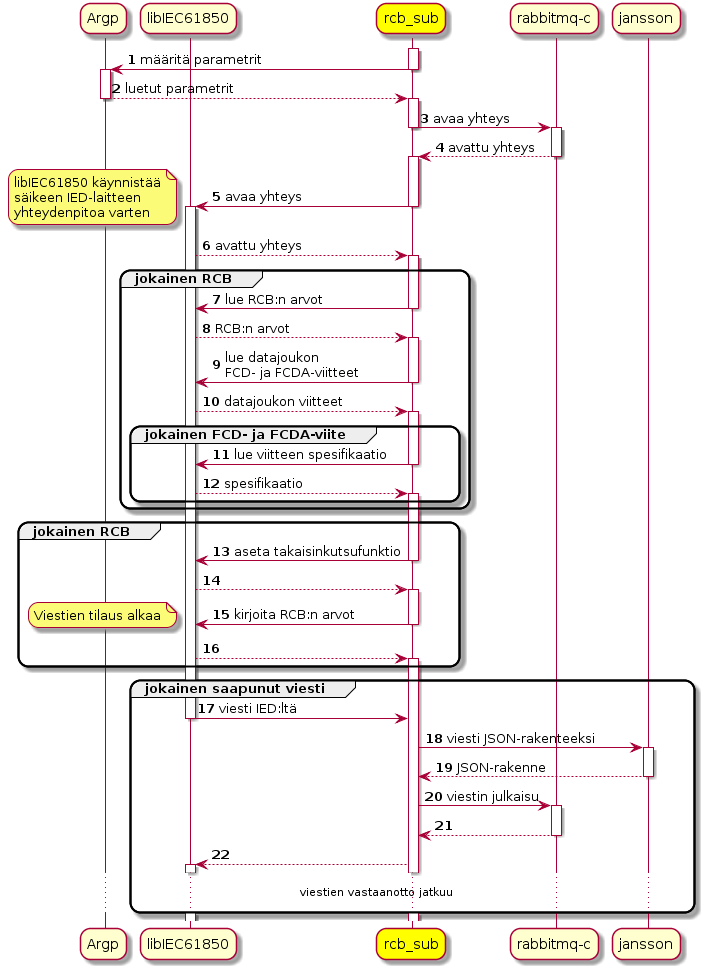
\includegraphics[width=1\textwidth]{pictures/rcb-sub-general-sd.png}
	\caption{Sekvenssikaavio rcb\_sub-ohjelman kokonaistoiminnasta.}
	\label{fig:rcb-sub-sekvenssikaavio}
\end{figure}


\section{Ohjelman toiminta}
\label{rcb-sub-toiminta}
Tulevissa kappaleissa käydään läpi yksityiskohtaisemmin rcb\_sub-ohjelman toimintaa, joka esiteltiin pääpiirteittäin kappaleessa \ref{ch:rcb-sub-yleiskuva}. Kappaleiden järjestys noudattaa kuvassa \ref{fig:rcb-sub-sekvenssikaavio} olevan sekvenssikaavion järjestystä. Toisin sanoen ohjelmaa käydään tarkemmin läpi sen suorituksen järjestyksessä.


\subsection{Parametrisointi}
Ohjelma parametrisoitiin Argp-kirjastolla. Kirjasto tarjoaa rajapinnan komentoriviparametrien käsittelyyn ja määrittämiseen. Parametrien muodot ovat tutut muista Linux-käyt\-tö\-jär\-jes\-tel\-män parametreista ja samaa periaatetta käytettiin tässäkin ohjelmassa. Kirjasto myös lisäsi ohjelmaan automaattisesti aputekstin käyttäjää varten. Aputeksti sisältää tietoa ohjelman parametreista ja niiden käytöstä. Aputekstin pystyi tulostamaan parametrilla \texttt{-{}-help}. Liitteessä \ref{ch:rcb-sub-help-output} on esitetty miltä ohjelman aputeksti näyttää. Liitteestä voi myös nähdä kaikki ohjelman parametrit ja lyhyen selityksen mihin kutakin käytetään.

Ohjelmiston parametrien voidaan ajatella koostuvan kolmesta eri ryhmästä. Ensin päätason vaihtoehtoiset parametrit \texttt{OPTIONS}. Pakolliset parametrit \texttt{EXCHANGE} ja \texttt{ROUTING\_KEY}. Viimeisenä n-kappaletta \texttt{RCB\_REF} ja \texttt{RCB\_OPTIONS} parametreja ryhmissä. Suurin osa \texttt{OPTION} parametreista on itsestäänselviä. Esimerkkinä \texttt{-{}-amqp-host}, joka kertoo A\-M\-Q\-P-pal\-ve\-li\-men IP-osoitteen, ja \texttt{-{}-ied-host}, joka kertoo IED-laitteen IP-osoitteen. Parametrit \texttt{EXCHANGE} ja \texttt{ROUTING\_KEY} määrittävät nimet RabbitMQ-palvelimen vaihteelle ja reititysavaimelle. Ryhmässä ensimmäinen \texttt{RCB\_REF} määrittää viitteen tilattavaan RCB-instanssiin IED-laitteella. Tätä seuraa vaihtoehtoinen \texttt{RCB\_OPTIONS} parametri. Se määrittää arvot, jotka kirjoitetaan edeltävä RCB-instanssille ennen tilausta. RCB-instanssin parametri \texttt{RCB\_OPTIONS} määrittää käytetyt vaihtoehtoiset kentät (\texttt{-{}-opt-fields}), käytetyt liipaisimet (\texttt{-{}-trigger}) ja pyydetäänkö yleistä kyselyä ennen muita viestejä (\texttt{-{}-gi}). Liipaisimet ja vaihtoehtoiset kentät asetetaan numeerisella arvoilla, jotka löytyvät myös aputekstistä (liite \ref{ch:rcb-sub-help-output}). Numeerisia arvoja voidaan summata yhteen, jotta voidaan asettaa monta arvoa yhtä aikaa. Liipaisimien nimet vastaavat aikaisemmin kappaleessa \ref{ch:rcb-toiminta} esitettyjä arvoja ja numeeriset arvot tulevat libIEC61850 -kirjastosta. Vaihtoehtoisten kenttien nimet vastaavat aikaisemmin taulukossa \ref{tab:iec61850-optional-fields-definition} esitettyjä arvoja ja numeeriset arvot tulevat myös libIEC61850-kirjastosta.

\subsection{Yhteyksien muodostus}
Parametrien luvun jälkeen ohjelma muodosti yhteydet ensin RabbitMQ-palvelimelle ja sen jälkeen IED-laitteelle. Kuvassa \ref{fig:rcb-sub-open-connections} on esitetty sekvenssikaavio, joka näyttä mitä kirjaston funktioita ohjelma kutsuu missäkin järjestyksessä. Funktiot ja niiden parametrit voi tarkemmin tarkistaa kirjaston omasta dokumentaatiosta. Tämä tarkentaa yleiskuvasta \ref{fig:rcb-sub-sekvenssikaavio} kohdat 3--6. Kaaviossa ohjelma muodostaa yhteydet vain kerran. Ohjelma on kuitenkin toteutettu niin, että se yrittää muodostaa yhteydet uudestaan vikatilanteissa. Jos muodostus ei onnistu, ohjelma kirjoittaa lokin tapahtuneesta ja odottaa hetken ennen uudelleen yritystä.

\begin{figure}[ht!]
	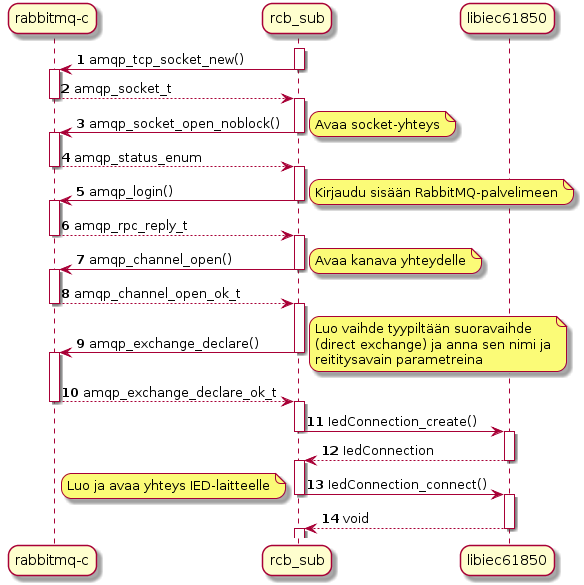
\includegraphics[width=1\textwidth]{pictures/rcb-sub-open-connections.png}
	\caption{Sekvenssikaavio kuinka rcb\_sub avaa yhteydet RabbitMQ-palvelimelle ja IED-laitteelle.}
	\label{fig:rcb-sub-open-connections}
\end{figure}

Yhteyden avauksen ja sisäänkirjautumisen jälkeen ohjelma avaa kanavan kohdassa 7--8. Kanava on yhteyden päälle avattu oma erillinen kommunikointiväylä, joka ei sotkeudu muihin kanaviin. Yhteen avattuun yhteyteen voi olla avattuna monta eri kanavaa. Kanavat mahdollistavat monen eri säikeen jakaa sama yhteys, ilman että tieto voi vuotaa toiseen säikeeseen. Kohdassa 9 kutsutaan funktiota \texttt{amqp\_exchange\_declare()}. Funktio määrittää vaihteen tyyppiä suoravaihde RabbitMQ-palvelimelle. Suoravaihde käsiteltiin kappaleessa \ref{ch:direct-exchange}. Ohjelmaan ei toteutettu parametria vaihdetyypin määrittämiseen, koska katsottiin että suoravaihde on riittävä nykyisten vaatimusten täyttämiseksi. Tulevaisuudessa voidaan tarvittaessa lisätä parametrit vaihdetyypin vaihtamiseen.


\subsection{IED:n attribuuttien tyyppin ja koon luku}
Yhteyksien muodostamisen jälkeen ohjelma käy läpi silmukassa jokaisen parametrina annetun RCB:n viitteen. Lukee RCB:n datajoukon viitteet ja selvittää jokaisen viitatun attribuutin spesifikaatiot, eli sen oikean viitteen, tyypin ja koon. Kuvassa \ref{fig:rcb-sub-reading-specifications} on esitetty sekvenssikaavio kuinka rcb\_sub tämän tekee libiec61850-kirjaston avulla. Kuva tarkentaa yleiskuvassa \ref{fig:rcb-sub-sekvenssikaavio} kohtia 7--12.

\begin{figure}[ht!]
	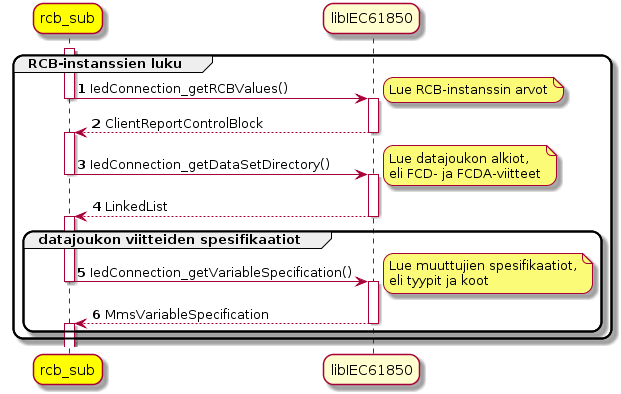
\includegraphics[width=1\textwidth]{pictures/rcb-sub-reading-specifications.png}
	\caption{Sekvenssikaavio kuinka rcb\_sub lukee RCB-instanssin arvot ja muuttujien spesifikaatiot.}
	\label{fig:rcb-sub-reading-specifications}
\end{figure}

Ensin RCB:sta luetaan sen tiedot IED-laitteelta (kohdat 1--2). RCB:ltä saadaan tieto mihin datajoukkoon se on liitetty. Tätä käsiteltiin kappaleessa \ref{ch:rcb-toiminta} ja taulukossa \ref{tab:iec61850-brcb-class-definition} kenttä \emph{DatSet}, joka kertoo käytetyn datajoukon viitteen. Tällä tiedolla ohjelma voi lukea datajoukon FCD- ja FCDA-viitteet (kohdat 3--4). Tästä saadaan jokainen viite listassa, joka käydään läpi silmukassa kohdissa 5--6. Jokaiselle viitteelle luetaan sen spesifikaatio. Spesifikaatiorakenne sisältää sisäkkäisiä spesifikaatioita, jos viite viittaa moneen muuttujaan IED-laitteen hierarkiassa. Tämä tapahtuu samalla periaatteella, jolla FCD- ja FCDA-viitteet viittaavaat moneen muuttujaan hierarkiassa alaspäin. Kuinka FCD- ja FCDA-viitteet toimivat käsiteltiin kappaleessa \ref{ch:fc-and-dataset}. Jokainen luettu viite tallennetaan ja niitä käytetään myöhemmin viestin kanssa JSON-rakenteessa. Esimerkkinä liitteessä \ref{ch:report-json-format} riveillä 21--22 tyyppi ja koko -tiedot.


\subsection{Viestien tilaus}
Ohjelman luettua kaikki muuttujien spesifikaatiot. Ohjelma tilaa silmukassa kaikki parametrina annetut RCB-instanssit. Kuvassa \ref{fig:rcb-sub-subscribe-reports} on esitetty sekvenssikaavio, kuinka rcb\_sub tilaa RCB-instanssit libiec61850-kirjaston avulla. Kuvan tarkentaa yleiskuvassa \ref{fig:rcb-sub-sekvenssikaavio} kohtia 13--16.

\begin{figure}[ht!]
	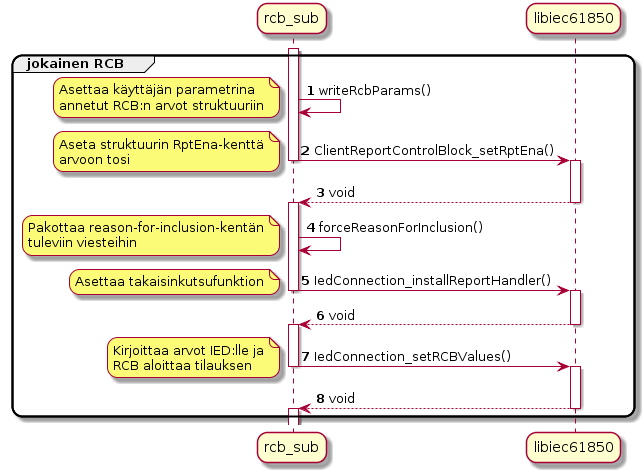
\includegraphics[width=1\textwidth]{pictures/rcb-sub-subscribe-reports.png}
	\caption{Sekvenssikaavio kuinka rcb\_sub tilaa RCB-instanssit.}
	\label{fig:rcb-sub-subscribe-reports}
\end{figure}

Ohjelma käsittelee libiec61850-kirjaston tarjoamaa \emph{ClientReportControlBlock} struktuurin instanssia. Kirjasto palauttaa struktuurin instanssin, kun RCB:n arvot luetaan IED-laitteelta. Kaikki RCB:lle kirjoitettavat arvot asetetaan instanssiin ennen IED-laitteelle kirjoitusta. Näitä arvoja ovat ohjelmalle parametreina annetut arvot, kuten liipaisimet ja vaihtoehtoiset kentät. Tämän ohjelma tekee kutsumalla omaa funktiota \texttt{wri\-teRcb\-Pa\-rams\-()} (kohta 1). Tämän jälkeen ohjelma asettaa RCB:n \emph{RptEna}-kentän arvoksi tosi (kohdat 2--3). Tämä kenttä kontrolloi RCB-instanssin varausta ja onko tilaus päällä. Seuraavaksi ohjelma pakottaa viestiin vaihtoehtoisen kentän \emph{reason-for-inclusion} (kohta 4). Tätä kenttää tarvitaan, jotta aikaisemmin luetut spesifikaatiotiedot saadaan yhdistettyä saapuneeseen viestiin. Tämän jälkeen asetetaan takaisinkutsufunktio, jota kirjasto kutsuu kun viesti saapuu (kohdat 5--6). Viimeisenä struktuurin arvot kirjoitetaan IED:llä olevalle RCB:lle (kohdat 7--8). Tämä varaa RCB-instanssin kirjoittavalle asiakkaalle, ja aloittaa tilauksen jos RptEna-kentän arvo oli tosi. RCB tulee lähettämään viestejä ohjelmalle samalla kun silmukan muilla kierroksilla käsitellään tilaamattomia RCB-instansseja.


\subsection{JSON:nin muodostaminen ja julkaisu}
Viestin saapuessa libiec61580-kirjasto kutsuu asetettua takaisinkutsufunktiota. Takaisinkutsufunktio muuttaa viestin JSON-muotoon ja lisäsi siihen aikaisemmin luetut muuttujien oikeat viittet, tyypit ja koot. Tämän jälkeen JSON-julkaistiin RabbitMQ-palvelimelle. Kuvissa \ref{fig:rcb-sub-report-to-json-1} ja \ref{fig:rcb-sub-report-to-json-2} on esitetty sekvenssikaaviolla kuinka ohjelma muuttaa viestin JSON:iksi ja julkaisee RabbitMQ:lle. Kuva \ref{fig:rcb-sub-report-to-json-1} jatkuu kuvassa \ref{fig:rcb-sub-report-to-json-2}. Kuva \ref{fig:rcb-sub-report-to-json-1} tarkentaa yleiskuvan \ref{fig:rcb-sub-sekvenssikaavio} kohtia 17--19 ja kuva \ref{fig:rcb-sub-report-to-json-2} kohtia 20--22.

\begin{figure}[ht!]
	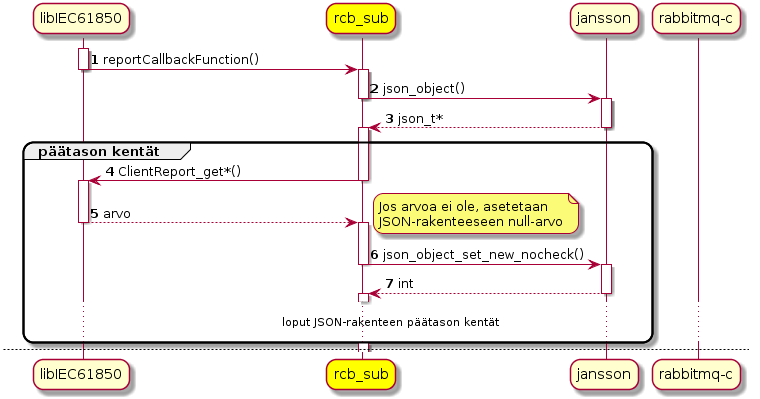
\includegraphics[width=1\textwidth]{pictures/rcb-sub-report-to-json.png}
	\caption{Sekvenssikaavio kuinka rcb\_sub muodostaa JSON:nin päätason kentät.}
	\label{fig:rcb-sub-report-to-json-1}
\end{figure}

Kuvassa \ref{fig:rcb-sub-report-to-json-1} suoritus alkaa kun libiec61850-kirjasto kutsuu takaisinkutsufunktiota. Funktiolle annetaan parametrina saapunut viesti \emph{ClientReport}-struktuurin instanssina (kohta 1). Tämän jälkeen ohjelma käy läpi viestin jokaisen päätason kentän ja lisää ne JSON-rakenteeseen. Osa viestin kentistä on vaihtoehtoisia riippuen siitä, mitä käyttäjä asetti \texttt{-{}-opt\--\-fields} parametrilla. Jos arvoa viestissä ei ole, korvataan se null-arvolla JSON:iin. Esimerkkinä liiteessä \ref{ch:report-json-format} rivillä 4 oleva \texttt{confRevision} muuttuja, jonka arvo on null. Tämän jälkeen suoritus jatkuu kuvasta \ref{fig:rcb-sub-report-to-json-1} kuvaan \ref{fig:rcb-sub-report-to-json-2}.

\begin{figure}[ht!]
	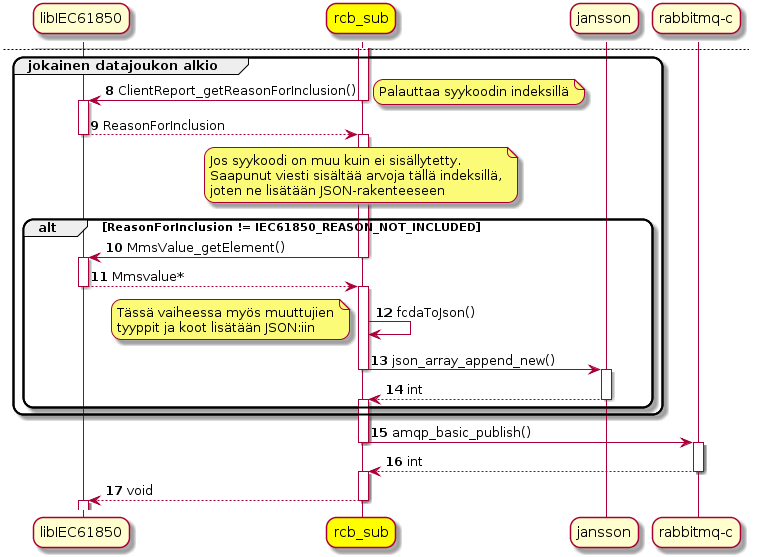
\includegraphics[width=1\textwidth]{pictures/rcb-sub-report-to-json_001.png}
	\caption{Sekvenssikaavio kuinka rcb\_sub lisää JSON:iin muuttujat viestistä.}
	\label{fig:rcb-sub-report-to-json-2}
\end{figure}

Päätason viestin kenttien jälkeen ohjelma käy läpi silmukassa viestin datajoukon indeksit (kuvassa \ref{fig:rcb-sub-report-to-json-2} kohdat 8--14). Viesti oikeasti sisältää vain ne datajoukon alkiot, jotka sisältyivät viestiin. Ongelmana tässä on se, että viesti ei sisällä indeksiä tai tietoa siitä mikä datajoukon alkio on kyseessä. Jotta tästä saadaan tieto, ohjelma pakottaa syykoodin päälle viestiin. Tämän avulla kun silmukassa käydään kaikki datajoukon indeksit läpi, voidaan jokaiselle indeksille ensin kysyä syykoodi viestistä (kohdat 8--9). Jos datajoukon alkio ei ole viestissä, palauttaa kirjaston funktio \texttt{Cli\-entRe\-port\-\_\-get\-Rea\-son\-For\-Inc\-lu\-si\-on\-()} arvon \texttt{IEC61850\_REASON\_NOT\_INCLUDED}. Tätä tietoa voidaan käyttää löytämään oikea datajoukon indeksi. Jos datajoukon indeksi on viestissä, suoritetaan kohdat 10--14, muuten mennään seuraavaan indeksiin ja toistetaan kohdat 8--9. Datajoukon indeksi tarvitaan, jotta aiemmin luetut spesifikaatiot saadaan yhdistettyä attribuutteihin arvojen kanssa. Datajoukon indeksillä, viestin arvoilla ja muuttujien tyypeillä ja koolla saadaan rakennettua loppuosa JSON-rakenteesta. Kuvassa \ref{fig:rcb-sub-report-to-json-2} oleva silmukka rakentaa liitteessä \ref{ch:report-json-format} olevan values-taulun alkaen riviltä 7. JSON:in sisempi values-taulu (rivi 13) on lista FCD- tai FCDA-viitteen muuttujia, mitä se viittaa arvoineen. Tämä taulukko muodostetaan kuvan \ref{fig:rcb-sub-report-to-json-2} kohdassa 12 funktiolla \texttt{fcdaToJson()} ja lisätään JSON:iin kohdassa 13. Lopuksi viesti lähetetään RabbitMQ-palvelimelle funktiolla \texttt{amqp\_basic\_publish()} ja takaisinkutsufunktio palaa (kohdat 15--17).

\section{Jatkokehitys}
Ohjelma jätettiin työssä pisteeseen, missä se saavutti kaikki sille asetetut vaatimukset. Kuitenkin tulevaisuudessa ohjelmaa voidaan lisätä ominaisuuksia tarpeen vaatiessa. Isoin puute ohjelmassa oli testiympäristö ja sen yksikkötestit. C:ssä ei ole suoraan tukea yksikkötestien kirjoittamiseen. Ympäristön pystytys vaatii erillisen kirjaston projektin yhteyteen, millä yksikkötestit kirjoitetaan. Tämä jäi tulevaisuuden kehitystyöksi ja ei sisältynyt tähän työhön. Yksikkötestit ovat kuitenkin tärkeä osa ohjelman ylläpitoa ja toiminnan varmistamista muutosten jälkeen. Testit tullaan tarvitsemaan ennemmin tai myöhemmin.

Ohjelma toteutettiin nyt niin, että se aina käyttää suoraa vaihdetyyppiä RabbitMQ-pal\-ve\-li\-mel\-la. Tämä täytti työlle asetetut vaatimukset. Jos tulevaisuudessa tarvitaan joustavuutta, voidaan ohjelmaan tehdä muutoksia ja parametreja lisätä helposti lisämään toiminnallisuutta. Esimerkkinä käyttäjä voisi valita käytettävän vaihteen tyypin parametrilla.
\chapter{Tulosten arviointi ja pohdinta}
\label{ch:arviointi}
Diplomityössä toteutettu ohjelma ei ole ollut tuotannossa osana muuta järjestelmää vielä kovin kauan. Kuitenkin tähän mennessä se on toiminut ongelmitta. Varmasti ei voida arvioida, että ohjelmassa ei tulisi ongelmia tulevaisuudessa, mutta ainakin alun perusteella tulokset näyttävät toimivilta. Tältä osin voidaan arvioida, että diplomityö pääsi asetettuihin tavoitteisiin onnistuneesti ja halutut vaatimukset saatiin täytettyä. Kuitenkin toimivuudesta huolimatta toteutuksessa on kohtia mitä voitaisiin parantaa, tehdä toisin ja jatkokehittää. Nämä ovat kuitenkin tulevaisuudessa yrityksen sisällä tehtäviä työtehtäviä tai mahdollisesti toisen diplomityön aiheita.

Työn aikana järjestelmän hajautukseen pohdittiin eri paradigmojen sopivuutta ja huomattiin, että siihen sopisivat julkaisija-tilaaja-, joukkokommunikointi- ja viestijono-pa\-ra\-dig\-mat. Toteutukseen valittiin AMQP-standardi, joka mahdollisti julkaisija-tilaaja- ja viestijono-pa\-ra\-dig\-mat, mutta ei suoraan ollut tarkoitettu joukkokommunikointiin. Tämän takia joukkokommunikointi jätettiin pois ja korvattiin julkaisija-tilaaja-paradigmalla. Kuinka hyvin joukkokommunikointi olisi sopinut toteutukseen ei ole tarkkaa tietoa. Kuitenkin julkaisija-tilaajan-paradigma jatkaa IEC 61850 -standardin määrittämää julkaisija-tilaaja-kom\-mu\-ni\-koin\-ti\-a IED-laitteen kanssa ja näin ollen sopii toteutukseen hyvin. Toteutukseen myös harkittiin MQTT-standardia AMQP:n sijaan, joka on pelkästään julkaisija-tilaaja-kom\-mu\-ni\-koin\-tiin tarkoitettu protokolla. Tämä valinta tehtiin tekijän aikaisemman kokemuksen ja muiden yrityksessä olevien henkilöiden keskustelun pohjalta. Koska joukkokommunikointi jätettiin pois toteutuksesta, olisi MQTT voinut sopia toteutukseen paremmin kuin AMQP sen keveyden takia.

IED-laitteelta tuleva viesti päätettiin muuntaa JSON-muotoon XML:än sijaan. Vertailua kahden välillä tehtiin ja päätös oli aikaisemmin tutkimuksen perusteella selvä. JSON-muoto on kevyempi kuin XML ja sopii viestin muotona hajautettuun järjestelmään. Suunniteltu JSON-rakenne on toimin	ut käytön ajan tarpeiden mukaan. Kuitenkin siinä olisi kohtia mitä pystyisi toteuttamaan toisin. Esimerkiksi \emph{bit-string} tyypin bittijärjestys (endian) voi vaihdella muuttujien välillä ja tämän takia siitä JSON-viestiin julkaistiin kaksi eri arvoa \emph{valueLittleEndian} ja \emph{valueBigEndian} (liite \ref{ch:report-json-format} rivit 23--24). Käytännössä vastuu muuttujan oikein lukemisesta siirretään tilaajalle. Standardissa kuitenkin on määritetty, kuinka päin muuttuja esitetään, jos se on tyyppiä bit-string. Tämän vastuun voisi mahdollisesti siirtää rcb\_sub-ohjelman puolelle ja tarjota JSON-viestissä pelkkä \emph{value}-kenttä, niin kuin kaikille muillekin muuttujille. Tämän lisäksi aikatyypit \emph{utc-time} JSON-viestissä päätettiin antaa siinä muodossa missä ne tulevat IED-laitteelta, eli millisekunteja UNIX-ajanlaskusta. JSON ei määritä käytettävää aikaformaattia, mutta JSON-rajapintoihin suositellaan käytettäväksi ISO 8601 -standardin aikaformaattia \cite{json-api-specification}.

Ennen varsinaista toteutusta demoon liittyviä ongelmien analyysista saatiin tuloksia suorituskykyyn liittyen. Näiden tietojen pohjalta ohjelman kieleksi valittiin C-kieli suorituskyvyn takia. Ongelmana demon suorituskyvyssä ei pelkästään ollut IED-laitteelta tulevien viestien määrä ja libIEC61850-kirjaston lukitus funktiokutsuissa. Todennäköisesti suurin syy oli Ruby-oletustulkin GIL, joka rajoittaa vain yhden säikeen suorituksen kerrallaan ja estää rinnakkaisuuden. C-kielen valinta oli hyvä ratkaisu. Ohjelman aika kaikkien RCB-instanssien tilaamiseen saatiin alas noin 30 sekunnista alle 15 sekuntiin. Suurin osa ajasta tulee IED-laitteille tehtävien kutsujen määrästä. Demon muistinkäyttö Ruby on Rails -ympäristössä oli noin 150 Mt. Rcb\_sub:in muistin käyttö saatiin noin 4 kt, joka on todella iso muutos aikaisempaan nähden. Tekniikan valinnan suhteen päätökset onnistuivat hyvin.

Ohjelman kehityksen aikana noudatettiin C-ohjelmoinnin ohjeistoa. Tarkoituksena välttää sen yleisimpiä virheitä, esimerkiksi tekstin formatointihyökkäys \cite{format-string-attack} ja muistin ylivuoto \cite{buffer-overflow-attack}. Tähän käytettiin apuna GCC-kääntäjän vipuja esimerkiksi \texttt{-Wall} ja \texttt{-Wextra} \cite{gcc-manual-warnings}. Huolellisesta ohjelmoinnista huolimatta järjestelmään tulee tietoa ulkopuoliselta IED-laitteelta, joka voi sisältää vahingollista tietoa. Tämä osuus jätettiin pois, koska se ei kuulunut tämän diplomityön aiheen piiriin. Tietoturvaa kuitenkin täytyy tarkistaa läpi tulevaisuudessa.

Järjestelmä aloittaa tilauksen käynnistämällä yhden rcb\_sub-prosessin per IED-laite. Tieto prosessille annettaan komentoriviparametreilla. Tilauksen muuttuessa, prosessi täytyy käynnistää uudelleen. Työn tekohetkellä ratkaisu sopi tarkoituksiin hyvin. Ratkaisuna olisi myös voinut toteuttaa yhden rcb\_sub-prosessin, joka pystyisi tilaamaan monta eri IED-laitetta rinnakkain, tai yhden IED-laitteen tilausta voisi muuttaa ilman, että prosessia täytyy käynnistää uudelleen. Tähän toteutustapaan tiedonsiirto komentoriviparametreilla ei enää onnistuisi vaan tarvittaisiin joku muu kommunikointitapa. Tähän sopisi aikaisemmin käsitellyt prosessien väliset kommunikointiparadigmat, esimerkiksi pistokkeet. Toteutuksessa monen eri rcb\_sub-prosessin tilaamat viestit ohjataan saman RabbitMQ-palvelimen kautta eri reititysavaimilla. Järjestelmän skaalautuessa isommaksi joutuu RabbitMQ isomman kuorman alle, joka todennäköisesti muodostuu pullonkaulaksi. Tarkkoja rajoja tähän ei vielä tiedetä ja nykyinen keskitetty RabbitMQ-palvelin todettiin riittäväksi tarkoituksiin tällä hetkellä. Kuitenkin tulevaisuudessa tämä on asia mikä täytyy ottaa huomioon.

Ohjelma jätettiin työssä pisteeseen, missä se saavutti kaikki sille asetetut vaatimukset. Kuitenkin tulevaisuudessa ohjelmaa voidaan lisätä ominaisuuksia tarpeen vaatiessa. Isoin puute ohjelmassa oli testiympäristö ja sen yksikkötestit. C:ssä ei ole suoraan tukea yksikkötestien kirjoittamiseen. Ympäristön pystytys vaatii erillisen kirjaston projektin yhteyteen millä yksikkötestit kirjoitetaan. Yksikkötestit ovat tärkeä osa ohjelman ylläpitoa ja toiminnan varmistamista muutosten jälkeen. Testiympäristön ja testien toteuttaminen jäi tulevaisuuden kehitystyöksi.

Tässä diplomityössä suunniteltu arkkitehtuuri ja ohjelmistoratkaisut toimisivat muissakin saman tyylisissä järjestelmissä, missä kommunikoidaan IEC 61850 -standardin mukaisesti ja tietoa julkaistaan eteenpäin. Periaatteessa suunnitelmasta olisi mahdollista toteuttaa oma kokonaisuutensa, jota olisi mahdollistaa käyttää muunkin järjestelmän kanssa. Tämä vaatisi kuitenkin tarkempaa suunnittelua ja edellä pohdittujen vaihtoehtojen käsittelyä.
\chapter{Yhteenveto}
\label{ch:yhteenveto}
% Diplomityön tuloksena saatiin ohjelmistokomponentti osaksi muuta sähköasemiin liittyvää järjestelmää.
Diplomityön tuloksena saatiin ohjelmistokomponentti osaksi isompaa sähköasemiin liittyvää järjestelmää. Komponentti kykeni tilaamaan viestejä IED-laitteelta IEC 61850 -stan\-dar\-din mukaisesti, muuntamaan viestit JSON-muotoon ja jakamaan sen muun järjestelmän kanssa. Viestien jako järjestelmässä toteutettiin AMQP-standardiin pohjautuvalla välittäjäpalvelimella, joka käyttää julkaisija-tilaaja- ja viestijono-kom\-mu\-ni\-koin\-ti\-pa\-ra\-dig\-mo\-ja. Toteutetun systeemin arkkitehtuuri esitettiin kuvassa \ref{fig:planned-system-architecture}. Arkkitehtuurissa muu järjestelmä on vastuussa tilauksien orkestroinnissa ja rcb\_sub-prosessien suorituksesta.

% Yhteenveto asetetuista vaatimuksista ja kuinka ne saavutettiin.
Diplomityön alussa asetettiin vaatimuksia jotka toteutuksen pitäisi pystyä täyttämään. Taulukossa \ref{tab:requirements-met} on esitetty yhteenveto asetetuista vaatimuksista ja kuinka ne tuontantoversiossa on täytetty. Taulukossa vaatimukset on esitetty niiden tunnuksilla, jotka asetettiin aikaisemmin kappaleessa \ref{ch:vaatimukset}.

\begin{table}[ht!]
	\caption{Yhteenveto asetetuista vaatimuksiin ja kuinka ne täytettiin.}
	\label{tab:requirements-met}
	\begin{tabular}{p{0.11\linewidth} | p{0.82\linewidth}}
		\hline
		\textbf{Vaatimus\-tunnus} & \textbf{Kuinka vaatimus täytettiin} \\
		\hline
		% viestien tilaus sähköasemalta IEC 61850 -standardin mukaisesti
		V1 & Viestit tilattiin käyttämällä libIEC61850-kirjastoa, joka hoitaa standardin mukaisen matalan tason kommunikoinnin. \\
		\hline
		% tilattujen viestien jakaminen järjestelmässä siitä kiinnostuvien komponenttien kanssa
		V2 & Viestien jakamiseen käytettiin viestijono- ja julkaisija-tilaaja-kommunikointiparadigmoja, jotka toteutettiin AMQP-standarin mukaisella RabbitMQ-välittäjäohjelmistolla. \\
		\hline
		% tilattuja viestejä haluavien komponenttien määrä pitää pystyä muuttumaan järjestelmän tarpeiden mukaan
		V3 & Komponentit pystyvät tilaamaan viestejä RabbitMQ-välittäjältä julkaisija-tilaaja-paradigman mukaan. Tilaajien määrää ei ole rajoitettu. \\
		\hline
		% muu järjestelmä ohjaa milloin viestien tilaus sähköasemilta aloitetaan ja lopetetaan
		V4 & Järjestelmä ajaa rcb\_sub-ohjelmaa taustaprosessina ja antaa tilauksen tarvittavat tiedot sille komentoriviparametreillä. \\
		\hline
		% komponenttien täytyy saada ilmoitus uudesta viestistä ilman erillistä kyselyä
		V5 & RabbitMQ-välittäjä tarjoaa ilmoituksen tilaajalle kun uusi viesti julkaistaan. \\
		\hline
		% viestit puskuroidaan myöhempää käsittelyä varten jos komponentti ei ehdi niitä heti käsitellä
		V6 & RabbitMQ-välittäjä tarjoaa viestijonoparadigman mukaisen jonon, jos tilaaja ei ehdi viestiä käsitellä. \\
		\hline
		% komponentin pitää pystyä suodattamaan viestit sen lähteen identiteetin perusteella
		V7 & Rcb\_sub julkaisee viestit RabbitMQ-välittäjälle IED-laitteen tunnisteella, jolloin tilaaja voi tilata haluamansa viestit. \\
		\hline
		% viestien jakamisen muoto pitää olla helposti ymmärrettävä järjestelmän osapuolien kesken
		V8 & IEC 61850 -standardin mukainen binääritason viesti muutettiin JSON-muotoon, joka on helpommin luettavissa ohjelmistolle ja ihmiselle. \\
		\hline
		% sähköasemalta tilattavien viestien määrä pitää pystyä muuttumaan tilauksien välillä
		V9 & Rcb\_sub-ohjelmaa ajetaan taustaprosessina ja järjestelmä voi muuttaa tilauksen tietoja (RCB-instassien määrä) syöttämällä eri komentoriviparametrit käynnistyksen yhteydessä. \\
		\hline
		% viestien välitystekniikka järjestelmässä täytyy tukea verkkopalvelun tapauksessa TCP/IP-protokollamäärityksiä
		V10 & MMS-protokolla ja valittu AMQP-standardi toimivat TCP/IP-protokollaperheen päällä. \\
		\hline
		% tiedonsiirrossa lähetystakuu ei ole välttämättömyys
		V11 & AMQP tarjoaa lähetystakuumekanismit julkaisijoiden ja tilaajien välille. \\
		\hline
	\end{tabular}
\end{table}

% Lähtökohtien avulla huomattiin että järjestelmän kommunikointiin tarvittiin viestijonoparadigma ja joukkokommunikointi tai julkaisija-tilaaja.
Työssä ratkaisua lähdettiin etsimään tarkastelemalla ensin hajautetun järjestelmän teoriaa, sen kommunikointiparadigmoja ja IEC 61850 -standardin määrityksiä. Saatuja tietoja apuna käyttäen suunniteltiin arkkitehtuuri osaksi muuta järjestelmää. Huomattiin, että viestijonoparadigma tarvittiin viestien puskurointiin ja kommunikointiin sopi jouk\-ko\-kom\-mu\-ni\-koin\-ti- tai julkaisija-tilaaja-paradigma.

% Toteutuksen tekniikaksi valittiin AMQP-standardi ja viesti päädyttiin muuntamaan JSON-muotoon.
Järjestelmän kommunikointiin valittiin AMQP-standardi, jonka myötä julkaisija-tilaaja-paradigma päätyi toteutukseen joukkokommunikoinnin sijaan. AMQP ei suoraan ollut tarkoitettu joukkokommunikoinnin toteuttamiseen. IEC 61850 -standardi määritti, että viestit IED-laitteelta tilataan julkaisija-tilaaja-paradigman mukaan. Toteutetun ohjelmiston ja valittujen paradigmojen voidaan sanoa jatkavan IED-laitteen tilausmekanismia ja näin ollen sopivat toteutukseen. Toteutus sallii monen tilaajan tilata sama viesti, mitä IEC 61850 -standardi ei ilman erillistä RCB-instanssia mahdollistanut. Viestin sisältö päädyttiin muuttamaan JSON-muotoon helpomman luettavuuden takia verrattuna MMS-protokollan binääriseen esitysmuotoon. Ohjelman tekemä JSON-muoto on nähtävissä liitteessä \ref{ch:report-json-format}. Edellä mainittujen pohjalta näiden osalta asetettuihin vaatimuksiin päästiin hyvin ja ne saatiin täytettyä. Nämä myös antavat vastaukset tutkimuskysymyksiin T1, T2 ja T3.

% Demon ongelmat ja niiden syyt.
Ennen diplomityön aloitusta tekijä oli yrityksessä toteuttanut demon ohjelmiston toimivuudesta. Demo oli tie oppia IEC 61850 -standardin toimintaa ja perehtyä aiheeseen tarkemmin ennen oikeaa toteutusta. Demossa oli kuitenkin ongelmia, mitkä haittasivat sen jatkokehitystä. Diplomityössä analysoitiin demon ongelmia, joita olivat huono suorituskyky, muistivuoto ja toiminnan epävarmuus. Toiminnan epävarmuuteen ja huonoon suorituskykyyn oli syynä Ruby-kielen oletustulkissa oleva globaali tulkkilukitus (GIL/GVL). Ja muistivuoto aiheutui huonosta Ruby-koodin ja C-kielen integraatiosta.

% Kuinka tekniset ongelmat ratkottiin toteutetussa ohjelmistossa.
Toteutetun ohjelman suorituskykyä saatiin paremmaksi valitsemalla matalamman tason C-ohjelmointikieli. C on käännettävä kieli verrattuna Ruby:n tulkattavaan kieleen. Lisäksi C voi hyödyntää käyttöjärjestelmän säikeitä ilman rajoituksia verrattuna Ruby-tulkin globaaliin lukitukseen. Muistivuoto saatiin korjattua huolellisella ohjelmoinnilla ja varmistamalla, että muisti vapautettiin, kun sitä ei enää tarvittu. Kielen valinnalla ohjelman muistinkäyttö saatiin entiseen nähden pienemmäksi. Ruby:llä toteutettu demo käytti muistia noin 150 Mt ja rcb\_sub käytti noin 4 kt. Toteutetussa ohjelmassa ei ollut demossa havaittavia ongelmia ja on osoittautunut tuotannossa toimivaksi muun järjestelmän kanssa. Edellä mainittujen perusteella demon analyysi onnistui ja sen pohjalta toteutukseen tehtiin oikeita teknisiä valintoja. Tämä myös vastaa tukimuskysymykseen T4.

% Toteutettu ohjelma on toiminut hyvin ja päästiin asetettuihin tavoitteisiin.
Toteutettu ohjelmisto on tuotannossa osana muuta järjestelmä ja diplomityön kirjoittamisen valmiiksi saamiseen asti on toiminut ongelmitta. Kappaleessa \ref{ch:arviointi} arvioitiin ja pohdittiin saatuja tuloksia. Näiden pohjalta voidaan sanoa, että diplomityössä suunniteltu toteutus pääsi asetettuihin tavoitteisiin ja tutkimuskysymyksiin löydettiin vastaus. Toteutus ei kuitenkaan ole täydellinen ja siinä on parannettavaa. Näihin kohtiin tullaan yrityksessä palaamaan tulevaisuudessa ja muuttamaan niitä, mikäli tarve vaatii. Tämän diplomityön tulokset tarjoavat myös apua samankaltaisten järjestelmien suunnitteluun ja toteutukseen.


% This adds used sources chapter.
\addto\extrasenglish{\btxifchangecaseoff} % Controls the case-changing for English titles. Make sure that case is preserved for abbreviations and proper nouns, e.g. title={The {ABC} of {Tex}: An Introduction to the Typesetting System}

\ifnameyear
  \bibliographystyle{babapaliktutnat}
\else
  \bibliographystyle{bababbrtut}
\fi
\bibliography{references}


% Starts the appendix part.
\appendix

% Include appendix chapters.
\chapter{Viestistä prosessoitu JSON-rakenne}
\label{ch:report-json-format}

\begin{lstlisting}[caption={Viestin prosessoitu JSON-rakenne.},label={lst:json-rakenne}]
{
  "dataSetName": "LD0_CTRL/LLN0$StatUrg",
  "sequenceNumber": 0,
  "confRevision": null,
  "timestamp": 1534993167923,
  "bufferOverflow": false,
  "values": [
    {
      "reasonForInclusion": "GI",
      "mmsReference": "LD0_CTRL/CBCILO1$ST$EnaCls",
      "reference": "LD0_CTRL/CBCILO1.EnaCls",
      "functionalConstraint": "ST",
      "values": [
        {
          "reference": "LD0_CTRL/CBCILO1.EnaCls.stVal",
          "type": "boolean",
          "value": false
        },
        {
          "reference": "LD0_CTRL/CBCILO1.EnaCls.q",
          "type": "bit-string",
          "size": 13,
          "valueLittleEndian": 0,
          "valueBigEndian": 0
        },
        {
          "reference": "LD0_CTRL/CBCILO1.EnaCls.t",
          "type": "utc-time",
          "value": 1534845456
        }
      ]
    },
    {
      "reasonForInclusion": "GI",
      "mmsReference": "LD0_CTRL/CBCSWI1$ST$Loc",
      "reference": "LD0_CTRL/CBCSWI1.Loc",
      "functionalConstraint": "ST",
      "values": [
        {
          "reference": "LD0_CTRL/CBCSWI1.Loc.stVal",
          "type": "boolean",
          "value": true
        },
        {
          "reference": "LD0_CTRL/CBCSWI1.Loc.q",
          "type": "bit-string",
          "size": 13,
          "valueLittleEndian": 0,
          "valueBigEndian": 0
        },
        {
          "reference": "LD0_CTRL/CBCSWI1.Loc.t",
          "type": "utc-time",
          "value": 1534845456
        }
      ]
    },
    {
      "reasonForInclusion": "GI",
      "mmsReference": "LD0_CTRL/CBCSWI1$ST$Pos",
      "reference": "LD0_CTRL/CBCSWI1.Pos",
      "functionalConstraint": "ST",
      "values": [
        {
          "reference": "LD0_CTRL/CBCSWI1.Pos.stVal",
          "type": "bit-string",
          "size": 2,
          "valueLittleEndian": 0,
          "valueBigEndian": 0
        },
        {
          "reference": "LD0_CTRL/CBCSWI1.Pos.q",
          "type": "bit-string",
          "size": 13,
          "valueLittleEndian": 2,
          "valueBigEndian": 2048
        },
        {
          "reference": "LD0_CTRL/CBCSWI1.Pos.t",
          "type": "utc-time",
          "value": 1534845480
        },
        {
          "reference": "LD0_CTRL/CBCSWI1.Pos.stSeld",
          "type": "boolean",
          "value": false
        }
      ]
    }
  ]
}
\end{lstlisting}
\chapter{C-ohjelman tulostama aputeksti}
\label{ch:rcb-sub-help-output}

\begin{lstlisting}[caption={rcb\_sub-ohjelman aputeksti.},label={lst:json-rakenne}, numbers=left]
Usage: rcb_sub [OPTION...]
	EXCHANGE ROUTING_KEY
	RCB_REF [RCB_OPTIONS...]
	[RCB_REF [RCB_OPTIONS...]...]
Configure and subscribe IED report control blocks.
Received reports are combined with variable specification
data and formatted to JSON. Formatted messages are
forwarded to AMQP broker using direct exchange.

 OPTION options:
  -a, --amqp-host=HOST       Host address of the AMQP
                             broker, defaults to localhost
  -e, --ied-port=PORT        Port for MMS communication,
                             defaults to 102
  -h, --ampq-vh=VH           Virtual host for the AMQP
                             broker, defaults to '/'
  -i, --ied-host=HOST        Host address of the IED,
                             defaults to localhost
  -m, --ampq-port=PORT       Port for AMQP communication,
                             defaults to 5672
  -p, --ampq-pwd=PWD         User password for the AMQP
                             broker, defaults to 'quest'
  -u, --ampq-user=USER       User for AMQP broker,
                             defaults to 'quest'
  -v, --verbose              Explain what is being done

 RCB_OPTIONS options:
  -g, --gi=VALUE             Set general interrogation
                             bit (1/0)
  -o, --opt-fields=MASK      Report optional fields int
                             bit mask (0 <= MASK <= 255)
  -t, --trigger=MASK         Report triggering int bit
                             mask (0 <= MASK <= 31)

  -?, --help                 Give this help list
      --usage                Give a short usage message
  -V, --version              Print program version

Mandatory or optional arguments to long options are also
mandatory or optional for any corresponding short options.

EXCHANGE is name of the exchange used with the AMQP
broker. ROUTING_KEY is routing key used for the
published AMPQ broker messages. RCB_REF is reference
to report control block as specified in IEC 61850 standard.
For example MY_LD0/LLN0.BR.rcbMeas01

Reason for inclusion optional field is set automatically
in order for the program to combine read specification
data and only to include needed data set values which
actually triggered the report.

Trigger MASK values:
  1  : data changed
  2  : quality changed
  4  : data update
  8  : integrity
  16 : general interrogation

Optional field MASK values:
  1   : sequence number
  2   : timestamp
  4   : reason for inclusion (automatically set, see above)
  8   : data set
  16  : data reference
  32  : buffer overflow
  64  : entry id
  128 : configure revision

Example usage:
$ rcb_sub -v -i192.168.2.220 testexchange testkey \
MY_LD0/LLN0.BR.rcbMeas01 -g1 -t27 -o16

Report bugs to mauri.mustonen@alsus.fi.
\end{lstlisting}

\end{document}